\documentclass[a4paper, 11pt, oneside]{report} 
\usepackage[utf8]{inputenc}
\usepackage[dutch]{babel}
\usepackage{diagbox}
\usepackage{amsmath}
\usepackage{amsfonts}
\usepackage{amssymb}
\usepackage{graphicx}
\usepackage{caption}
\usepackage[table,xcdraw]{xcolor}
\usepackage[toc,page]{appendix}
\usepackage{hyperref}
\usepackage{titlesec}
\usepackage{listings}
\usepackage{float}
\usepackage{tikz}
\usetikzlibrary{trees}
\usepackage{tikz-qtree}
\usepackage{graphicx}
\usepackage{fancyref}
\usepackage{wrapfig}
\usepackage{url}
\usepackage{pdflscape}
\usepackage{fancyvrb}
\usepackage{fancyhdr}
\graphicspath{ {Afbeeldingen/} }
\usepackage{subfig}
\usepackage{tabularx}
\usepackage{apacite}
\usepackage{longtable}
\usepackage{titlecaps}
%\usepackage[T1]{fontenc}
\usepackage{titlesec, blindtext, color}
\definecolor{gray75}{gray}{0.75}
\newcommand{\hsp}{\hspace{20pt}}
\usepackage{pdfpages}
\usepackage{booktabs}
\usepackage{listings}

\newcolumntype{L}[1]{>{\raggedright\arraybackslash}p{#1}}

\titleformat{\chapter}[hang]{\huge\bfseries}{\thechapter\hsp\textcolor{gray75}{|}\hsp}{0pt}{\Large\bfseries}

\makeatletter
\newcommand\tagreq[2]{#1\def\@currentlabel{#1}\label{#2}}
\makeatother

\def\checkmark{\tikz\fill[scale=0.4](0,.35) -- (.25,0) -- (1,.7) -- (.25,.15) -- cycle;} 
\def\figureautorefname{Figuur}
\def\subsectionautorefname{Subparagraaf}
\def\sectionautorefname{Paragraaf}
\def\chapterautorefname{Hoofdstuk}
\def\tableautorefname{Tabel}
\DeclareRobustCommand{\VAN}[3]{#2} % set up for citation

%% Sets page size and margins 
\usepackage[a4paper,top=3cm,bottom=3cm,left=3cm,right=3cm,marginparwidth=1.75cm]{geometry}

\definecolor{dkgreen}{rgb}{0,0.6,0}
\definecolor{gray}{rgb}{0.5,0.5,0.5}
\definecolor{mauve}{rgb}{0.58,0,0.82}

\lstset{frame=tb,
	language=C++,
	aboveskip=3mm,
	belowskip=3mm,
	showstringspaces=false,
	basicstyle=\footnotesize,% basic font setting
	backgroundcolor=\color{black!3}, % set backgroundcolor
	columns=flexible,
	basicstyle={\small\ttfamily},
	numbers=none,
	numberstyle=\tiny\color{gray},
	keywordstyle=\color{blue},
	commentstyle=\color{dkgreen},
	stringstyle=\color{mauve},
	breaklines=true,
	breakatwhitespace=true,
	tabsize=3
}

\author{M.W.J. Berentsen}
\font\myfont=cmr12 at 40pt
\title{\myfont Drone meshnetwerk simulatie}
\usepackage{titling}

\newcommand{\subtitle}[9]{%
	\posttitle{%
		\par\end{center}
	\begin{center}\large#1\end{center}
	\begin{center}\large#2\end{center}
	\vskip0.5em
	\begin{center}\normalsize#3\end{center}
	\begin{center}\large#4\end{center}
	\begin{center}\large#5\end{center}
	\begin{center}\large#6\end{center}
	\begin{center}\normalsize#7\end{center}
	\begin{center}\normalsize#8\end{center}
	\begin{center}\normalsize#9\end{center}
	\vskip0.5em}%
	\rfoot{{\footnotesize \textbf{#1}}}
}

\subtitle{Afstudeerverslag}{Versie 2.0}{Alten Nederland B.V.}{Hogeschool van Arnhem en Nijmegen}{HBO Technische Informatica - Embedded Software Developement }{MWJ.Berentsen@student.han.nl}{Studentnummer: 561399}{Docent: J. Visch, MSc}{Assessor: ir. C.G.R. van Uffelen}

\setlength{\parindent}{0pt}
\setlength{\parskip}{5pt plus 2pt minus 1pt}



\hypersetup{colorlinks=true, urlcolor=red,citecolor=black,linkcolor=blue}  % Colours hyperlinks in blue, but this can be distracting if there are many links.
\setcounter{tocdepth}{2}

\usepackage{fancyhdr}
\pagestyle{fancy}

\setlength\headheight{26pt} %% just to make warning go away. Adjust the value after looking into the warning.
% \rhead{{\color{blue}\rule{1cm}{1cm}}}

\rhead{
\includegraphics[height=1cm]{Afbeeldingen/han.png}}



\begin{document}
\begin{figure}
\begin{center}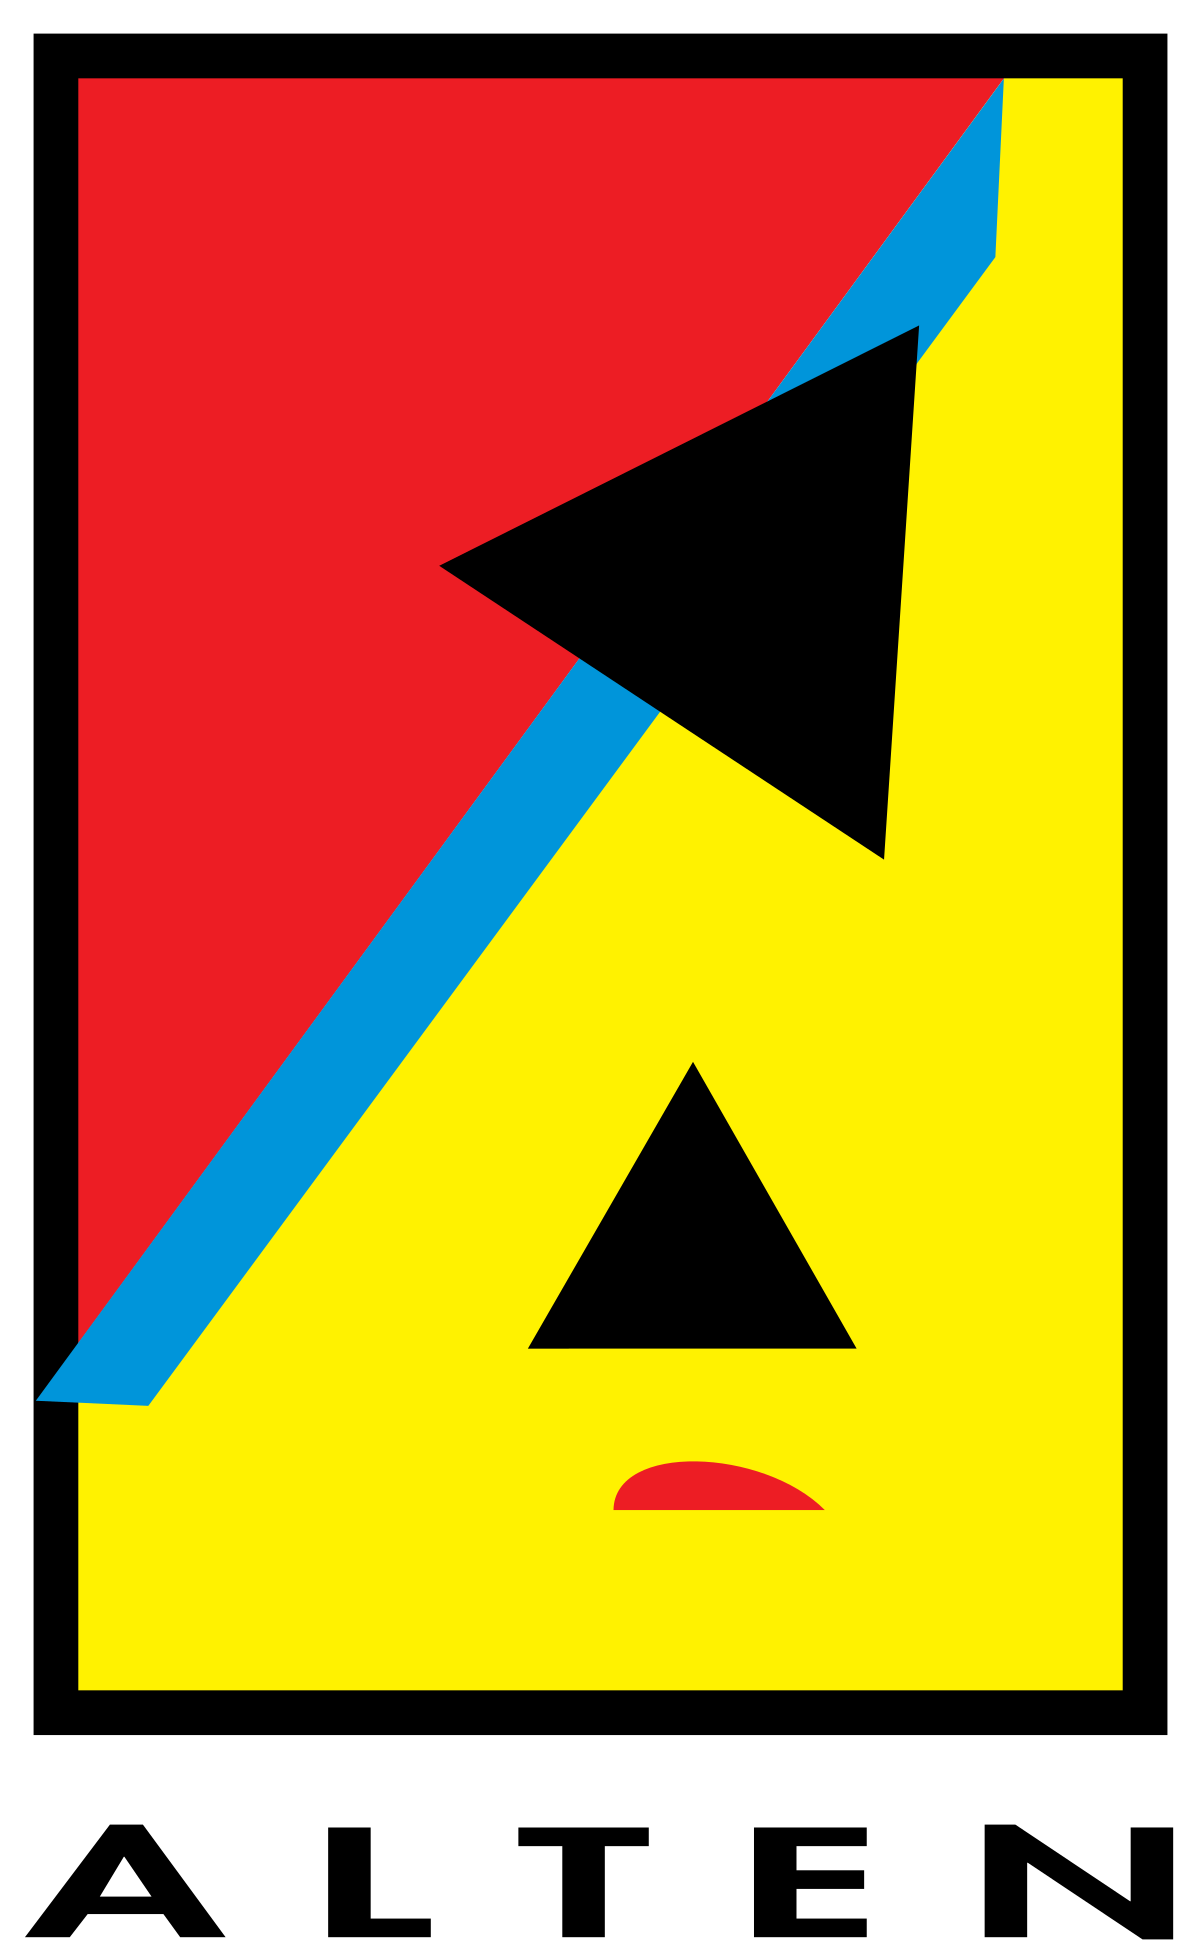
\includegraphics[scale=0.1]{alten}\end{center}
\end{figure}
\maketitle

%\section*{Voorwoord}
%\addcontentsline{toc}{section}{\protect\numberline{}Voorwoord}
%\pagebreak
\chapter*{Managementsamenvatting}\label{sec:managementsamenvatting}
Het doel van ``Drone meshnetwerk simulatie"\ is het zetten van de eerste stap in de ontwikkeling van het dronenetwerk. Hiervoor is de volgende opdracht opgesteld:
\begin{quotation}
	\textit{Maak een netwerkmodule voor een drone die het mogelijk maakt om meerdere drones onderling te voorzien van een zelf herstellend meshnetwerk. Maak deze module na in een simulatie die geschikt is om meer dan 100 drones te simuleren, waarvan het netwerk zich gelijk gedraagt zodat er verdeelalgoritmes getest kunnen worden.}
\end{quotation}

%Deze opdracht is uitgevoerd door eerst literatuur onderzoek te doen.

Eerst is er gekeken welke simulatiesoftware gebruikt moet worden voor het simuleren van het dronenetwerk.
Er is gekozen om dit te doen in de softwarecombinatie Ros + Gazebo omdat dit het hoge aantal drones kan verwerken en ook toegang heeft tot een physics engine.

Om een betere keuze te kunnen maken welke hardware gebruikt zou moeten worden voor onderlinge communicatie, is er eerst gekeken wat de grootte van de payload is die verstuurd zou moeten worden om nuttig te zijn in een netwerk.

Vervolgens is gekeken naar welke hardware gebruikt zou moeten worden voor de onderlinge communicatie. Hier is gekozen voor een Raspberry Pi model 2B+ met een daarop aangesloten radio module de nRF24l01+.

Hierna is er een keuze gemaakt welke routeringstechniek gebruikt moet worden waarop de conclusie was om een hybride routeringstechniek te gebruiken. Deze techniek heeft als basis een reactief protocol met als toevoeging dat richtingen opgeslagen worden in plaats van routes. De student heeft een aangepaste versie van de Lightweight Mobile Routing Protocol(LMR) toegepast. 

Er is een conclusie getrokken dat het voor dit project niet nodig is om een drone volledig te implementeren. Er zijn regels opgesteld waar een drone minimaal aan zou moeten voldoen om een abstracte drone te representeren. 

Om de opdracht uit te kunnen voeren heeft de student een simulatie gemaakt waar drones zich kunnen voortbewegen en zich conform de casus kunnen verdelen. De drones volgen het gedrag van een meshnetwerk en er is applicatie aanwezig om op realistische wijze verzoeken te sturen naar de drones voor verplaatsing. 

De opgeleverde software wordt onderbouwd in het software design document en de software requirements specificatie.

Concluderend is er een simulator opgeleverd waarin drones verdeeld kunnen worden.
Deze simulator kan gebruikt worden om te experimenteren met verdelingen en netwerkgedrag.
Daarnaast is er een fysiek prototype opgeleverd van een netwerkmodule die zich gelijk gedraagt als de gesimuleerde netwerkmodule en via een REST service aangestuurd kan worden.   

\tableofcontents
\clearpage
\chapter*{Begrippenlijst}
\label{inleiding:begrippenlijst}

\begin{longtable}[c]{|l|l|}
	\hline
	\rowcolor[HTML]{9B9B9B} 
	Term & Beschrijving \\ \hline
	\endhead
	%

%	Adapter & \begin{tabular}[c]{@{}l@{}}Een ontwerppatroon die gebruikt wordt om niet passende \\interfaces op elkaar aan te sluiten.\end{tabular} \\ \hline
	Broadcast & Het rond sturen van een bericht die iedereen mag ontvangen. \\ \hline
%	Byte & Een samenstelling van 8 bits. \\ \hline
	Debug & \begin{tabular}[c]{@{}l@{}}Term die slaat op debugger, vaak informatie die gebruikt \\ wordt om gedrag te vinden binnen een applicatie.\end{tabular} \\ \hline
	Gateway & Een toegangspunt tot een netwerk. \\ \hline
	Gazebo & Simulatiesoftware met ondersteuning voor physics. \\ \hline
	nRF24l01+ & Radio transciever module werkzaam op de 2,4Ghz band. \\ \hline
	Physics engine & Software die natuurwetten toepast op virtuele objecten. \\ \hline
	\begin{tabular}[c]{@{}l@{}}Raspberry Pi \\ model 2B+\end{tabular} & Micro computer geschikt voor prototyping. \\ \hline
	Ros & \begin{tabular}[c]{@{}l@{}}Robot operating system. Wordt gebruikt voor de transportlaag \\ naar zowel virtuele als gesimuleerde robots.\end{tabular} \\ \hline
	Rosservice & Een request response mechanisme gebruikt door Ros nodes. \\ \hline
	Rostopic & Publicatie voor het gebruik van een subscriber patroon binnen Ros. \\ \hline
%	Router & Netwerkcomponent die berichten kan doorsturen. \\ \hline
	Routeringstechniek & \begin{tabular}[c]{@{}l@{}}Techniek die gebruikt voor het opbouwen van een pad binnen\\ een netwerk.\end{tabular} \\ \hline
	RQT & Programma aangeboden door Ros voor aansluiting op Ros nodes. \\ \hline
	SDF & \begin{tabular}[c]{@{}l@{}}XML format gebruikt voor het inladen van objecten en werelden\\ in gazebo\end{tabular} \\ \hline
	Seriële verbinding & Een communicatieverbinding het meest bekend van USB. \\ \hline
	Simulatie software & Software die fysieke objecten nabootst in software. \\ \hline
%	Unittest & Geautomatiseerde test die functie test op resultaat. \\ \hline
	\caption{Begrippenlijst.}
	\label{tab:begrippenlijst}\\
\end{longtable}


\chapter{Inleiding}\label{sec:inleiding}

Dit document is het eindverslag van de afstudeeropdracht genaamd "Drone meshnetwerk simulatie".
De simulatie simuleert een netwerk van drones die onderling met elkaar verbonden zijn door het gebruik van meshnetwerk technieken.
De simulatie dient een tweevoudig doel: Allereerst kunnen er met de simulatie verdeelalgoritmes getest worden. Het tweede doel is het simuleren van het netwerk om zo de stabiliteit hiervan te kunnen optimaliseren.

Het doel van dit document is het aantonen van de volwassenheid van het project en de opgeleverde deelproducten conform de vijf beroepscompetenties.
Dit wordt bewezen aan de hand van de producten die zijn gerealiseerd of handelingen die zijn verricht tijdens de afstudeerstage. In dit document wordt regelmatig verwezen naar andere documenten zoals het plan van aanpak, onderzoekrapport, software design document en de software requirements. Dit wordt gedaan omdat deze documenten ook aantonen dat de student zich HBO waardig heeft gedragen tijdens dit project.  

Het eindverslag is zo opgebouwd dat dit de opdracht, context en eindproducten beschrijft en hoe de student bezig is geweest conform de vijf beoordelingscriteria.

\begin{itemize}
	\item Bedrijfsbeschrijving.
	
	Hier wordt het bedrijf omschreven waar de opdracht wordt uitgevoerd en het team wordt besproken.
	\item Opdrachtomschrijving.
	
	Dit hoofdstuk wordt gebruikt om de aanleiding, probleemstelling, doel, opdracht en resultaten toe te lichten.
	
	\item Methoden, technieken, platforms, tools.
	
	De gebruikte methoden, technieken, platforms en tools worden in dit hoofdstuk toegelicht. Hier gaat het met name om waarom er een keuze is gemaakt en wat de alternatieven waren. De projectmanagement methodiek blijft hierbuiten aangezien deze al wordt toegelicht in het plan van aanpak.
	
	\item Uitvoer projectplan.
	
	Hier wordt het plan van het project gereflecteerd. Er wordt gekeken wat er volgens planning ging maar wat ook niet en waarom dat dan zo was.
	
	\item Proces en aanpak
	
	In het hoofdstuk proces en aanpak wordt er gekeken welke stappen zijn genomen en wat hun verband is met betrekking tot het proces
	
	\item Resultaten
	
	Wat is er opgeleverd en voldoet het aan de opgestelde kwaliteitseisen gesteld in het plan van aanpak. Als er afwijkingen zijn worden die ook in dit hoofdstuk besproken.
	
	\item Evaluatie 
	
	Dit hoofdstuk geeft inzicht met betrekking tot het proces, producten en resultaten en het functioneren van de student.
	
	\item Conclusie
	
	Het afsluitende hoofdstuk behandeld wat de student heeft opgeleverd en of dit voldoet aan de doelstelling van het project.
	Als er afwijkingen zijn wordt dit ook beschreven.
	Tenslotte worden er een advies gegeven aan het bedrijf in welke vervolgstappen zij zou kunnen nemen.
	
\end{itemize}

\chapter{Bedrijfsbeschrijving}\label{sec:bedrijfsbeschrijving}

Alten is een multinational met +- 25.000 medewerkers wereldwijd en is van origine begonnen in 1988 en in de eerste tien jaar organisch gegroeid totdat ze in 1999 een beursgenoteerd bedrijf werden.
Vanaf het jaar 2000 hebben ze de eerste internationale dochterondernemingen gestart waarvan de eerste in Nederland in 2002 was (dit was een overname van een ander bedrijf).
In 2005 is Alten NL tot leven geroepen die zich focust op het geven van technische consultancy.
Op dit moment heeft Alten NL ongeveer 650 medewerkers, waarvan elk persoon minimaal een bachelors diploma heeft, 30-40\% een masters diploma, en 10-15\% een PhD heeft.
Dit maakt Alten een vooruitstrevend bedrijf die zich altijd bezig houdt met innoverende technologieën en probeert vooraan te staan wanneer er een nieuwe technologie doorbreekt.

Anno 2019 heeft Alten vier filialen in Nederland: Amstelveen, Capelle a/d IJssel, Eindhoven en Apeldoorn.
De student is geplaatst bij het filiaal in Apeldoorn.

Zoals gezegd focust Alten zich vooral op technologie en dat is niet enkel beperkt tot software want zo hebben ze namelijk ook: Technische Software, mechatronica, IT test services, Business Intelligence \& Analytics en Digital Enterprise.
Alten faciliteert voornamelijk in consultancy (85\% van alle werkzaamheden) maar doen ook ‘in huis’ projecten voor haar klanten.

Het bedrijf heeft zes kernwaarden die als volgt luiden: kennisnetwerkers, technologie, streef hoog, open en betrokken, mensen en plezier/lol.
Alten benadrukt dat het belangrijk is om je kennis te delen met anderen (want samen sta je sterker), dit proberen zij te bereiken met de zogeheten kennisgroepen. 

\section{Het team}\label{sec:het-team}
Het team betrokken bij dit project wordt hier kort omschreven.

\paragraph{Uitvoerend student: Maurice Berentsen}

Het afstudeerproject is uitgevoerd door de student Maurice Berentsen. 
Hij is een student aan de Hogeschool van Arnhem en Nijmegen. 
Zijn belang bij dit project is tweezijdig. 
Enerzijds voert Maurice dit project uit om aan te tonen hij de vijf beroepscompetenties beheerst en daarom waardig is voor het ontvangen van het Bachelor diploma Technische Informatica. 
Anderzijds voert hij dit project uit omdat hij een interesse heeft naar mobiele meshnetwerken en dit na het behalen van zijn diploma in de praktijk zou willen brengen bij een toekomstig opdrachtgever. 

\paragraph{Technisch manager: Hugo Logmans}

Hugo Logmans is de technische manager voor Alten oost. Hij begeleidt de consulenten in hun carrière en werk. Sinds 1999 is Hugo werkzaam als ontwikkelaar en heeft hier dus bijna 20 jaar ervaring in. Zijn belang in dit project is het onderzoeken wat er toegevoegd kan worden in een meshnetwerk om het ondervinden van uitgevallen punten snel te achterhalen.

\paragraph{Business manager: Jeroen Nijenhuis}
Jeroen Nijenhuis is business manager van de locatie oost. Hij zorgt voor contactafhandeling naar bijvoorbeeld p\&o. Bij hem kan de student terecht voor vragen buiten het vakgebied. Zijn belang bij het project is het zorgen dat de overgang van de schoolomgeving naar een bedrijfsomgeving goed verloopt 

\paragraph{Bedrijfsbegeleider: Hugo Heutinck}

Hugo Heutinck is een werknemer van Alten. Hij heeft in 2003 een master behaald in Computer Technics en is sindsdien aan het werk als (embedded) software engineer. Hij is een specialist in Linux en heeft voert de rol uit van SCRUM master. Zijn belang bij dit project is het begeleiden van de student.

\paragraph{Begeleidende leraar: Jorg Visch}
 
Jorg Visch is een leraar op de Hogeschool van Arnhem en Nijmegen werkzaam binnen het lerarenteam van de uitstroomrichting Embedded Software Developer. Hij is leraar van Maurice geweest tijdens het semester Internet of Things. Zijn belang bij dit project is begeleiden van Maurice tijdens het afstuderen.

\paragraph{Assessor: Chris van Uffelen}

Chris van Uffelen is een collega van Jorg Visch en werkzaam in hetzelfde team. Hij heeft Maurice begeleidt tijdens het Object-oriented Software and Modelling project. Zijn belang bij dit project is het beoordelen of het project waardig is aan het verschaffen van het Bachelor diploma Technische Informatica. Hij doet dit in samenwerking met Jorg Visch. 


\chapter{Opdrachtomschrijving}\label{sec:opdrachtomschrijving}
Het doel van Alten is om onderling verbonden drones te kunnen verdelen om zo een netwerk op te kunnen bouwen over een gebied. 
Alten wil dat dit netwerk zichzelf kan onderhouden door te reageren op uitval of een slechte verbinding door de één of meerdere drones te herverdelen.

\section{Probleem}\label{sec:probleem}
Op dit moment is Alten in het bezit van drones maar deze kunnen niet met elkaar communiceren.
Om te kunnen communiceren moet er een netwerkmodule toegevoegd worden aan elke drone.
Alten wil grote netwerken kunnen opbouwen die robuust zijn en daarom wil zij gebruik maken van een zelf herstellend meshnetwerk.
Hoewel er al meerdere oplossingen bestaan in het gebruik van meshnetwerken wil Alten het zelf herstellend vermogen vergroten. 
Daarom wil Alten dat de focus van de netwerkmodule ligt op het snel detecteren van uitval van punten in het netwerk zodat daar adequaat op gereageerd kan worden.
Adequaat reageren kan op twee manieren volgens Alten.
De netwerkmodule kan een ander netwerkpunt zoeken om via dat punt te communiceren, als deze niet beschikbaar is het alternatief om de drones opnieuw te verdelen.
Het autonoom fysiek kunnen verplaatsten van de netwerkpunten is dan ook de uitbreiding die Alten wil toevoegen aan het zelf herstellend vermogen.
Alleen wat is een efficiënte manier van herverdelen?
Het makkelijkste is om alle drones terug naar hun start punt laten vliegen maar dit zou betekenen dat het netwerk op dat moment niet beschikbaar is en het zou ook nog eens onnodig veel stroom verbruiken.

Om algoritmes te testen voor het verdelen van de drones is een simulatie de oplossing.
Hierbij is het dus ook van belang dat een simulatieomgeving zich realistisch gedraagt. 
Om realistisch gedrag na te bootsen moeten de virtuele netwerk modules zich in de simulatie zich net zo gedragen als in het echt.

\section{Doelstelling}\label{sec:doelstelling}
Het doel van dit project is het zetten van de eerste stap in de ontwikkeling van het dronenetwerk.
De eerste stap is ontwikkelen van een netwerkmodule voor het onderling verbinden van drones.
Het is van belang dat het meshnetwerk van de drones snel kan reageren op uitval van netwerkpunten.
Deze netwerkmodule moet zowel virtueel als fysiek gerealiseerd worden in dit project.

Voor het virtueel realiseren van de netwerkmodule moet een simulatie gebruikt worden. 
Omdat er nog geen simulatiesoftware beschikbaar is wil Alten dat de student uitzoekt welke simulatiesoftware geschikt is voor het simuleren van meer dan 100 drones.
Vervolgens kan de student deze software gebruiken om de virtuele netwerkmodules te testen.

\section{Opdracht}\label{sec:opdracht}
De opdracht van dit project is de ontwikkeling van meerdere producten die bijdragen aan het behalen van het doel. 

De student moet een prototype maken van een netwerkmodule die het onderlinge meshnetwerk verzorgt en zichzelf kan herstellen bij uitval of slecht signaal.
Wanneer er geen alternatieve communicatie route mogelijk is moet de module de drone een instructie uitsturen om zich te herpositioneren.

De student moet een simulatie opzetten waarin de netwerkmodules verplaatst kunnen worden in een vrije ruimte. 
In de simulatie moet het mogelijk zijn om de netwerkmodules te verplaatsen aan de hand van hun $X$, $Y$ en $Z$ as zodat er verdeelalgoritmes getest kunnen worden.  
De netwerkmodules moeten in de simulatie kunnen uitvallen en de onderlinge afstand heeft effect op de virtuele signaalsterkte.
De simulatie moet aan de hand van een script herhaalbaar zijn met eenzelfde resultaat.

Alten wil graag dat de simulatiesoftware gebruik maakt van Robot Operating System (Ros) als middleware. 
Dit wil Alten omdat zij al kennis heeft in Ros maar nog niet in combinatie met drones en meshnetwerken en door het begeleiden hier ervaring in opdoet.
Het ervaring opdoen in Ros is geen doel van dit project en de student hoeft zich hier niet op te concentreren.

Hoewel de keuze van de simulatiesoftware zich concentreert op het simuleren van een dronenetwerk zal de student alleen de netwerkmodule toevoegen aan de simulatie. 
De student zal zich dus niet specialiseren in het realistisch simuleren van drones.

Het project is geslaagd als een prototype van het meshnetwerk is opgeleverd samen met een simulatie waarin het meshnetwerk getest kan worden met verschillende verdelingsalgoritmes.

\subsection{Casus}\label{sec:casus}
Om het doel waar naartoe gewerkt moet worden te voorzien van een richting heeft Alten een casus bedacht.
Deze casus wordt hieronder toegelicht in een schets en is voorzien van individuele situaties.
Er wordt gedrag omschreven voor een simpel algoritme van het herstel van het meshnetwerk om aan te tonen dat dit getest kan worden in de simulatie.
In de casus blijft het vlieggedrag buiten de scope.


In de schets van \autoref{fig:schetsNetwerk} wordt er vanuit gegaan dat elke drone een directe vluchtroute heeft met zijn verbonden netwerkpunt.
De verbindingen zijn gemaakt  om de casus uit te leggen en volgen dus niet de realistische verbindingen die ze zouden hebben op basis van locatie.
\begin{figure}[H]
	\begin{center}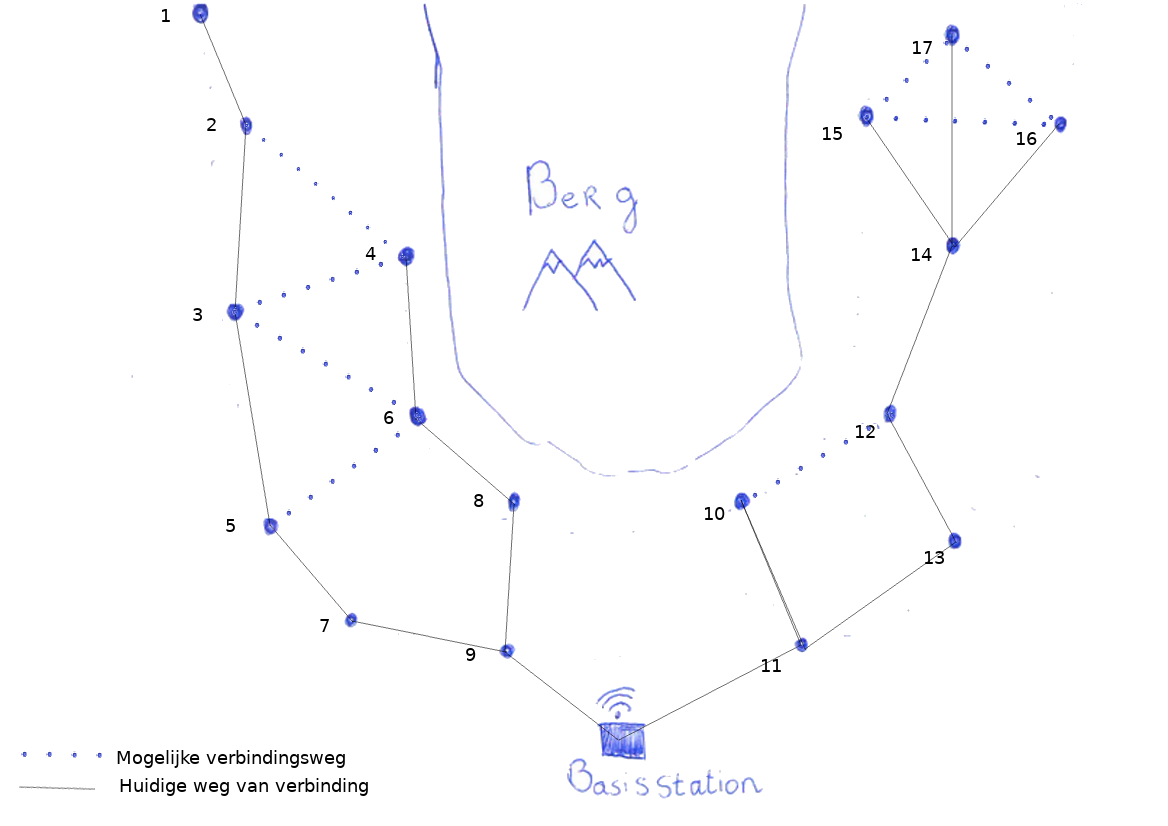
\includegraphics[width=0.61\linewidth]{schetsNetwerk}\end{center}
	\caption{Schets van casus netwerk.}
	\label{fig:schetsNetwerk}
\end{figure}
In de casus komen de volgende situaties apart voor:

\begin{itemize}
	\item Punt 2 valt uit waardoor punt 1 geen verbinding meer heeft met het basisstation. Het verwachte resultaat is dat drone 1 zich verplaatst naar de positie van drone 2 en zo het netwerk herstelt.
	\item De bovenstaande situatie gebeurd. Tijdens het verplaatsen van punt 1 herstelt punt 2 zich weer. Het verwachte resultaat is dat punt 1 weer terug  keert naar zijn oude positie.
	\item Punt 3 valt uit waardoor punt 1 en 2 geen verbinding meer hebben met het basisstation. Het verwachte resultaat is dat drone 2 een nieuwe verbinding aangaat met drone 4.
	\item Punt 14 valt uit waardoor punt 15, 16 en 17 geen verbinding meer hebben met het basisstation. Het verwachte resultaat is dat de drones 15, 16 en 17 eerst met elkaar verbinden, vervolgens zal één van de drones zich verplaatsen naar punt 14. 
\end{itemize}

\section[Op te leveren resultaten]{Op te leveren resultaten voor het bedrijf en school}\label{sec:op-te-leveren-resultaten-voor-het-bedrijf-en-school}

Aan het einde van het project levert de student de volgende producten op aan het bedrijf:

\begin{itemize}
	\item Simulatiesoftware met netwerksimulatie
	\item Prototype meshnetwerk module.
	\item Broncode van de bovenstaande producten. 
	\item SRS (Software Requirement Specification)
	\item SDD (Software Design Document)
	\item Onderzoeksverslag
\end{itemize}

Aan het einde van het project levert de student het bovenstaande plus een projectverslag op aan de Hogeschool van Arnhem en Nijmegen.


\chapter{Methoden, technieken, platforms, tools}\label{sec:methoden-technieken-platforms-tools}
%Wat gebruik je en waarom, overwogen alternatieven, waarom is de keuze gevallen op die
%tool/techniek/platform. En dan niet zozeer (of alleen) de project(management)methodiek, die is al
%uitgebreid verantwoord in het PvA als het goed is.
Dit hoofdstuk wordt gebruikt om de methoden, technieken, platforms en tools toe te lichten.

\section{Github naast Alten haar eigen Git server}

Gedurende het project is gebruik gemaakt van een dubbele git server voor versiebeheer.
Hiervoor is een private repository op github.com gebruikt en de de aangeboden server van Alten.

Deze keuze is gemaakt omdat het afstudeerproject een belangrijk project is. 
Daarom is het belangrijk dat het aantal single points of failure zo laag mogelijk blijft.
Om een werknemer van Alten te citeren:``Je kan gerust alleen gebruikt maken van onze server daar is nooit wat mee'' bleek toch het tegendeel zie \autoref{fig:servernietbeschikbaar}

\begin{figure}[H]
	\begin{center}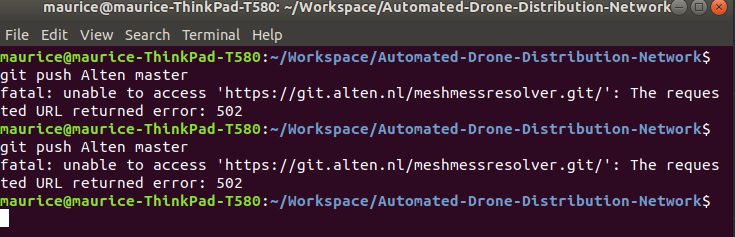
\includegraphics[width=0.61\linewidth]{Afbeeldingen/AltenGit.png}\end{center}
	\caption{Alten server niet beschikbaar.}
	\label{fig:servernietbeschikbaar}
\end{figure}

Toen dit gebeurde was de keuze om niet afhankelijk te zijn van een enkele service terwijl dit niet hoeft een bewezen goede keuze.

\section{Game engine}

Tijdens het project is gebruik gemaakt van de simulatiesoftware Gazebo. Deze softwarekeuze is gebaseerd op het onderzoek die van te voren is uitgevoerd en wordt daar ook ruim onderbouwt. Een alternatief die ik niet in het onderzoek heb meegenomen maar nog wel hier wil aankaarten is de overweging om een game engine te gebruiken. Deze keuze heb ik voor het onderzoek overwogen mee te nemen omdat game engine geavanceerde physics bevatten en gemakkelijk te gebruiken zouden zijn voor prototyping. Daarnaast heb ik voor het afstuderen begon de minor GAME gedaan waardoor ik ook al de nodige ervaring heb in het werken met game engines. De reden dat ik uiteindelijk de keuze niet meegenomen heb in het onderzoek is omdat ik wist dat game engines niet geschikt zijn om code te verwerken die zonder al te veel moeite ook op een microcontroller werken. Daarnaast zou het gebruiken van een game engine ook niet passen in mijn uitstroomrichting als embedded software developer.

\section{Redmine}

Voor het bijhouden en plannen van het project is gebruik gemaakt van een Redmine omgeving. 
De keuze om deze te gebruiken is gekomen door positieve de ervaring opgedaan met Redmine tijdens het Internet of Things semester.
Een overwogen alternatief was het gebruiken van Github projects omdat deze een gemakkelijkere koppeling zou hebben naar de commits op git dan Redmine heeft. Ook zou de service van Github projects betrouwbaarder zijn dan de door Alten gehoste Redmine server.

De keuze om toch de Redmine server van Alten te gebruiken is gebaseerd op het volgende:
\begin{itemize}
	\item Inzichtelijker voor mijn begeleiders vanuit Alten. 
	\item Standaard geïntegreerde Gantt planning.
	\item Mogelijkheid voor sprint planningen.
	\item Bij uitval is de planning tijdelijk niet inzichtelijk dit wordt niet als kritisch beschouwd.  
\end{itemize}   


\section{\LaTeX}

De keuze om Latex te overwegen in het project is al bijna twee jaar voor het afstuderen begon gemaakt. 
Toen de leraar Joost Kraaijeveld tijdens het semester World of Robots de mogelijkheden liet zien van Latex is er in eigen tijd meer aandacht gestoken in de markup taal.
Het werd duidelijk dat Latex de tool was voor het schrijven van wetenschappelijke artikelen of technische documentatie.
Hier kwam uit dat Latex veel voor je kan automatiseren zoals referenties, bibliografie, betiteling en het opstellen van formules maar dat er wel een leercurve bij zit.
Om te voorkomen dat ik tijdens het afstuderen nog door die leercurve heen zou moeten gaan ben ik toen al begonnen met kleine documenten te schrijven in Latex voor opdrachten van semesters.
Toen ik dit meer onder knie had heb ik besloten ook mijn verslag voor de meewerkstage te schrijven in Latex.
Tijdens de stage werd door alle begeleiders aangegeven dat het verslag er zeer netjes en verzorgd uitziet.
Ook heb ik tijdens de meewerkstage ondervonden dat deze tool veel geschikter is voor versiebeheer dan de concurrent Microsoft Word.

Tijdens het afstuderen is Word ook geen praktisch alternatief omdat het project uitgevoerd wordt met Ubuntu. 
Daarop kan geen Word geïnstalleerd worden waarbij de linux variant van LibreOffice overblijft of de online tool van Word.

Omdat ik deze beide geen waardig alternatief vond ten opzichte van Latex waar ik ondertussen aardig bekwaam in ben heb ik definitief besloten tijdens het afstuderen om Latex te gebruiken

\section{Template formulieren gebruik}

Tijdens de eerste fase van het project is er het plan geweest om templates te gebruiken gedurende het project.
Hiervoor was gekozen omdat het tijdens het WoR project veel gemak opleverde. 

Met het afstuderen kwam ik er al snel achter dat bepaalde templates voor dit project niet nodig waren.
Zo is er een template waar de planning van de komende iteratie in opgeschreven moest worden te vinden in bijlage \ref{app:Iteratieplan}.
Dit template is uiteindelijk niet gebruikt, er is al vrij snel de overstap gemaakt om de planning in Redmine bij te houden zoals te zien in \autoref{fig:sprint2}.

\begin{figure}[H]
	\begin{center}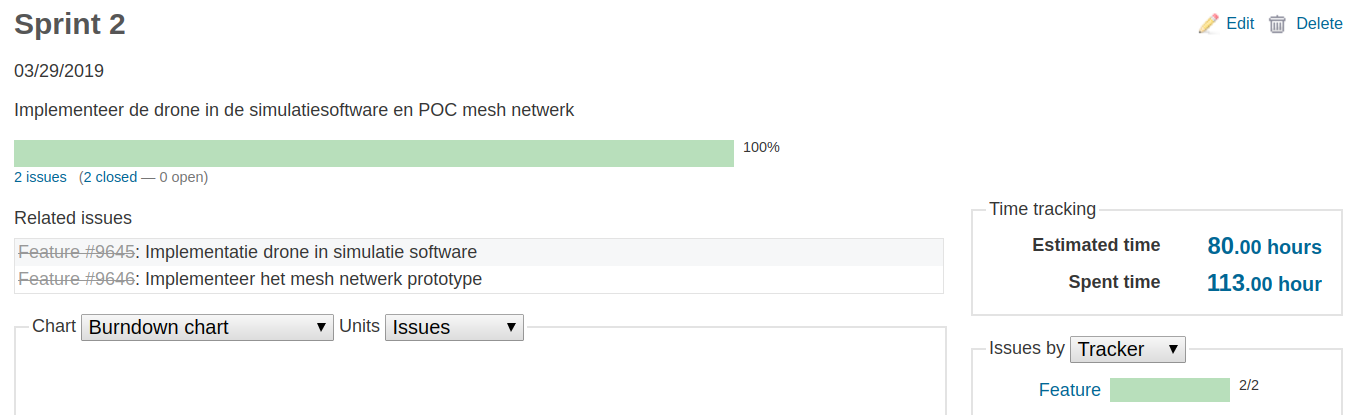
\includegraphics[width=1\linewidth]{Afbeeldingen/sprint2.png}\end{center}
	\caption{Redmine sprint 2 planning.}
	\label{fig:sprint2}
\end{figure}

Mijn begeleiders waren niet altijd op locatie en door het registeren van de planning in Redmine was er snel en gemakkelijk overzicht in de sprintplanning.

Een template die eigenlijk ook voortvloeit uit de hiervoor beschreven template is het IterationAssessment uit bijlage \ref{app:IterationAssessment}.
De sprints zijn veel informeler afgesloten door het er gewoon mondeling over te hebben met de begeleider tijdens de lunch of de koffietafel.
Achteraf was het niet zo slim om het op deze manier af te sluiten zonder dat ook op schrift vast te leggen.
Ik denk dat dit een valkuil is voor studenten die afstuderen omdat ze toch vaker alleen aan een opdracht werken.
Hoewel er stakeholders waren tijdens het project die natuurlijk ook op een later moment besproken stof willen kunnen teruglezen is het er niet gekomen.
Dit is een fout geweest van mij die er ingeslopen is.
In een volgende project wil ik daarom dus ook absoluut hier verandering in brengen en daar de tijd nemen om meer vast te leggen.   

Een ander template die wel gebruikt is, is de template voor een usecase te vinden in bijlage \ref{app:Usecase}.
Dit template heeft veel gemak opgeleverd tijdens het SDD (bijlage \ref{app:SoftwareDesignDocument}). 
Omdat er al een template aanwezig was heb ik mij volop kunnen concentreren op wat er toe doet en dat is het opstellen van de usecase. 



\section{Template Vector3 class}

Tijdens het bouwen van de software van het netwerkcomponent is begonnen met het maken van software voor de simulatie.
Vanuit gemakzucht is er op dat moment gebruik gemaakt van de bestaande Vector3 die meegeleverd wordt met ROS \cite{ignitionVector}.
Op dat moment was het een gemakkelijke oplossing zodat er snel verder gewerkt kon worden. 

Later toen de software ook moest draaien kwam de afhankelijkheid terug naar voren die gecreëerd was.
Er is gekozen om de vector3 zelf te implementeren in een template klasse aangezien niet alle functionaliteit van de vector3 uit de iginition libary\cite{ignitionVector} gebruikt wordt.
Om specifiek te zijn wordt er zelfs maar een enkele functie gebruikt voor het bepalen van een afstand tussen twee vectoren.
Die is als volgt in de code geïmplementeerd. 

\begin{lstlisting}
template <typename T>
float Vector3<T>::Distance(const Vector3<T>& rhs) const
{
Vector3<T> difference(*this);
difference -= rhs;
return std::sqrt( std::pow( difference.X(), 2 ) + std::pow( difference.Y(), 2 ) + std::pow( difference.Z(), 2 ) );
}
\end{lstlisting}

In deze functie wordt de stelling van Pythagoras gebruikt om de afstand tussen twee vector punten te berekenen.

Door het maken van deze klasse is de code van het netwerkcomponent onafhankelijk geworden van externe libaries.

\section{CppCheck}
Tijdens het project is gebruik gemaakt van een statische code checker.
De keuze was gevallen op de CppCheck vanwege het gebruikersgemak.
Bij oplevering toont de tool geen melding meer, deze zijn onderdrukt of opgelost.
De resultaten van CppCheck zijn te vinden in bijlage \ref{sec:resultaat-cppcheck}.


\section{GoogleTest}

Gedurende het project is er gebruik gemaakt van unit testen. 
Deze testen zijn geschreven via het framework GoogleTest.
Dit leverde toen er op een later moment een template class van een 3D vector (bijlage \ref{app:broncode}/drone\_meshnetwork\_simulation/src/Vector/) gemaakt werd het voordeel dat deze test driven ontwikkeld kon worden.  
Verder is de mogelijkheid van testen gebruikt om de opslag van routerichtingen te verifiëren en het coderen van berichten te testen.
Een uitdraai van de de unittesten is terug te vinden in bijlage \ref{sec:resultaten-googletest}

\section{CMake}
Aan het einde van het project heeft de gesimuleerde software de overstap gemaakt naar het fysieke prototype. 
Hiervoor moest de code gecompileerd worden op een Raspberry Pi.
In de simulator werd ik als ontwikkelaar natuurlijk al een beetje verwend door het standaard aanwezige catkin  in ros.
Tijdens het compileren van de code op de Raspberry Pi kwam ik eerst nog weg door telkens een lang commando in te voeren waarmee het router programma werd aangemaakt.
Later toen er ook nog een gateway programma aangemaakt moest worden heb ik besloten om een overstap te maken naar CMake \cite{cmake}.

Hierdoor kon ik door een enkel commando beide programma's simpel compileren op de Raspberry Pi.
Dit bewees zijn nut helemaal op het moment toen er getest moest worden met meerdere Raspberry Pi's.

\chapter{Uitvoer projectplan}\label{sec:uitvoer-projectplan}
In de dit hoofdstuk wordt het plan eerst kort toegelicht, vervolgens wordt gekeken naar waar de afwijkingen zitten en waarom deze er waren.

%Wat was het plan, hoe heb je dat uitgevoerd. Waar zitten de afwijkingen en waarom? Beperkt tot inhoudelijk relevante zaken.


\section{Het plan}\label{sec:het-plan}
Het plan is om dit project volgens de RUP ontwikkelmethode uit te voeren. 
Omdat er nog niet voldoende voorkennis aanwezig is voor het bouwen van de software geeft dit de ruimte om voldoende onderzoek uit te voeren en daar de kennis uit te halen. 
Er is gepland dat de fases inception, elaboration, construction en transition een duur hadden van vijf, acht, vier en twee weken. Dit geeft de student dusdanig veel tijd voor onderzoek en het opzetten van losse prototype componenten dat er tijdens een constructiefase van 4 weken weinig problemen kunnen voorkomen. 

In de eerste fase de inception fase is gepland dat er een plan van aanpak geschreven wordt en dat er ruimte is voor kleine onderzoeken waarvan de resultaten meteen meegenomen kunnen worden in de planning van het te komen onderzoek.
Vervolgens tijdens de elaboratie fase staat het onderzoek naar de te gebruiken hardware voorop omdat hier de te bouwen simulatie op gebaseerd moet worden.    
Op het moment dat de hardware bekend is kan deze wanneer nodig besteld worden en wordt er gekeken naar welke simulatiesoftware gebruikt moet worden.
Als ook dit bekend is is de volgende stap het bouwen van losse componenten in de simulatie. 
Zodra de hardware beschikbaar is kan de software die voor simulatie gemaakt is gebruikt worden op de hardware.
In de constructiefase kon de gebouwde software en hardware gebruikt worden voor het beantwoorden van onderzoeksvragen. 
Ook zou er in deze fase van het project voldoende tijd moeten overblijven voor het afronden van de documentatie.
Tenslotte zou er in de transitiefase ruimte zijn voor het maken en geven van presentaties voor school en het bedrijf
 
\section{Reflectie}\label{sec:reflectie}

Zoals bij de meeste projecten is dit project anders verlopen dan gepland is. Zo begon het met de tegenvaller dat er veel meer aandacht naar het plan van aanpak moest dan verwacht was. Hierdoor was er minder tijd om kleine onderzoeksvragen uit te voeren die wel van belang waren in voor de onderzoeken in de elaboratiefase. Hierdoor moesten deze doorgeschoven worden.

Omdat er een onduidelijkheid zat wat er opgeleverd moet worden bij de 80\% versie, wat beter omschreven wordt in \autoref{sec:altijd-navragen-nooit-aannemen}, werd er in week drie van de elaboratie fase besloten dat er nieuwe planning gemaakt moest worden om aan de vraag van school te voldoen. 
Hier is besloten dat het beter zou zijn dat het hardware prototype pas gebouwd zou worden na het inleveren van de 80\% versie als de beschikbare tijd het ook toestaat. 
De focus is verschoven naar het bouwen van een correct werkende simulatie die af is voor  de 80\% versie.
Het deel van het onderzoek dat al uitgevoerd is, bevatte genoeg handvatten voor het bouwen van alle software. 
Daarom is deze ontwikkeling ook meteen gestart en is de software stapsgewijs opgebouwd. Hoe dit gedaan is wordt omschreven in \autoref{sec:constructiefase}. 

Dit wijkt af van de RUP methodiek waarbij componenten los van elkaar gebouwd worden en waar de construction fase gebruikt wordt om deze componenten op elkaar aan te sluiten. Dit besluit is genomen wegens de harde deadlines uit het project. Het direct op elkaar aansluiten van de componenten tijdens het schrijven van de software kan wanneer correct uitgevoerd tijd schelen maar brengt het risico met zich mee dat componenten gaan afwijken in hun interface. Deze keuze kon alleen gemaakt worden door het feit dat het afstudeerproject alleen wordt uitgevoerd waardoor er altijd genoeg kennis is van alle componenten en interfaces.

Concluderend kan gesteld worden dat voor dit project RUP de juiste ontwikkelmethode is ondanks dat het verkeerd is uitgevoerd. 
Het onderzoek van te voren naar de te gebruiken technieken heeft de kennis opgeleverd welke nodig is voor het project. Tijdens de elaboratiefase en de constructiefase zijn de regels van RUP wellicht geschonden, maar net als elke methode zijn de regels niet in steen gehouwen.
Door het flexibele optreden is wel een werkend product neergezet die het doel verzadigd van Alten terwijl de student ook zijn doel heeft behaald in het bewijzen dat hij bekwaam is als embedded software engineer. 
 

\chapter{Proces en aanpak}\label{sec:proces-en-aanpak}
%Wat heb je gedaan en waarom? Wat is het verband tussen de verschillende stappen die je genomen hebt in
%het proces?
In dit hoofstuk wordt het proces en de aanpak van het afstudeerproject omschreven.
In het project is gewerkt met de RUP ontwikkelmethodiek, aan de hand van deze fases worden de verschillende stappen van het project doorgelopen.

\section{Inceptiefase}\label{sec:inceptiefase}

Aan het begin van het afstudeerproject is een plan van aanpak (projectplan) opgesteld met input vanuit Alten.
Dit plan is toegevoegd als bijlage \ref{app:bijlage:plan-van-aanpak}
Om achter de eisen en wensen van Alten te komen zijn middels meerdere gesprekken het probleem en doel van de opdracht geanalyseerd om deze concreet te beschrijven.
Voor dit onderdeel waren meerdere gesprekken nodig, omdat de achtergrond van het project in eerste instantie niet concreet omschreven was.
Door de meerdere gesprekken met Alten is de opdracht geconcretiseerd. De geconcretiseerde opdracht is te lezen bij \autoref{sec:opdrachtomschrijving} \nameref{sec:opdrachtomschrijving}.

Voor het schrijven van het plan van aanpak was vijf weken ingepland. 
In eerste instantie werd geschat dat die dusdanig veel tijd was dat er tijdens deze fase al begonnen kon worden aan kleine onderzoeken.
De reden hierachter was het idee dat de uitkomst van deze kleine onderzoeken zou helpen in het inschatten van een planning.

Doordat het concept plan nog niet concreet genoeg was heeft dit meer aandacht en tijd nodig gehad dan verwacht. 
Hierdoor zijn de volle vijf weken van de inceptiefase gebruikt om tot een kwalitatief plan te komen voor het project.

\section{Elaboratiefase}\label{sec:elaboratiefase}

De elaboratie fase is begonnen met het opstellen van een software requirements specificatie(SRS) te vinden in bijlage \ref{app:softwarerequirementspecification}.
Dit kon gedaan worden met de requirements van de opdrachtgever uit het plan van aanpak en het doorvragen aan de opdrachtgever.
Door het vooraf maken van dit document werd de opdracht verder geconcretiseerd.
Deze requirements konden weer meegenomen worden in het onderzoeksverslag als criteria in keuzes.  
Er is rekening mee gehouden dan er bepaalde eisen aan de software pas duidelijk zouden worden gedurende het onderzoek.
Vandaar dat het schrijven van de onderzoeken en het schrijven van een SRS enige overlap zou hebben. 

Het schrijven van het onderzoek, bijlage \ref{sec:onderzoeksrapport-drone-meshnetwerk-simulatie}, is begonnen met het opdelen van van de hoofdvraag in meerdere deelvragen. 
Deze deelvragen zijn vervolgens ingepland als taken op het scrum bord in Redmine.
Deze taken zijn vervolgens in sprints afgerond. 
Dit betekend dat er in iteraties van twee weken gewerkt is. 
De onderzoekstaken zijn van te voren al toegewezen aan een specifieke sprint.
Bij het begin van elke sprint zijn de taken geconcretiseerd.
Deze keuze is gemaakt omdat  veel taken in het project de kennis vereisen van de taak ervoor.


Er is het besluit gemaakt om de elaboratiefase met vier weken te verkorten. 
Dit besluit is gemaakt omdat het duidelijk werd dat het belangrijk was dat er bij de zogeheten 80\% versie van het project een product op te leveren die al voldoende is om op af te studeren. 
Er is op dat moment voldoende kennis uit het onderzoek aanwezig om een goede simulatie te kunnen schrijven die zich zou houden aan de limieten van de te gebruiken hardware. 
Meegenomen in het besluit was dat de HAN zelf ook een hogere prioriteit heeft op softwareontwikkeling dan het onderzoek ook al moeten ze wel beiden aanwezig zijn.

Daarom heeft de laatste week van de elaboratie fase in het teken gestaan van het op orde maken van het Software Design Document te vinden in bijlage  \ref{app:softwarerequirementspecification}.
Deze week is ook de eerste week dat er code geschreven is. 
Dit was vaak code die bestond uit lege classes of kleine stukjes proef code zoals het uitproberen hoe een abstracte drone geplaatst kon worden in Gazebo.

\section{Constructiefase}\label{sec:constructiefase}
Het voorgaande besluit hield in dat er nog zes weken de tijd was om de simulatie te realiseren voor de 80\% versie ingeleverd moest worden.
\paragraph{Abstracte gesimuleerde drone}
Er is begonnen met het ontwikkelen van een abstracte drone die voorzien is van een interface  om aangestuurd te worden zich te verplaatsen naar verschillende locaties.
Een abstracte drone houdt in dat alles wat niet van belang is weglaten mag worden daardoor bleef er alleen blokje over.
\begin{figure}[H]
	\begin{center}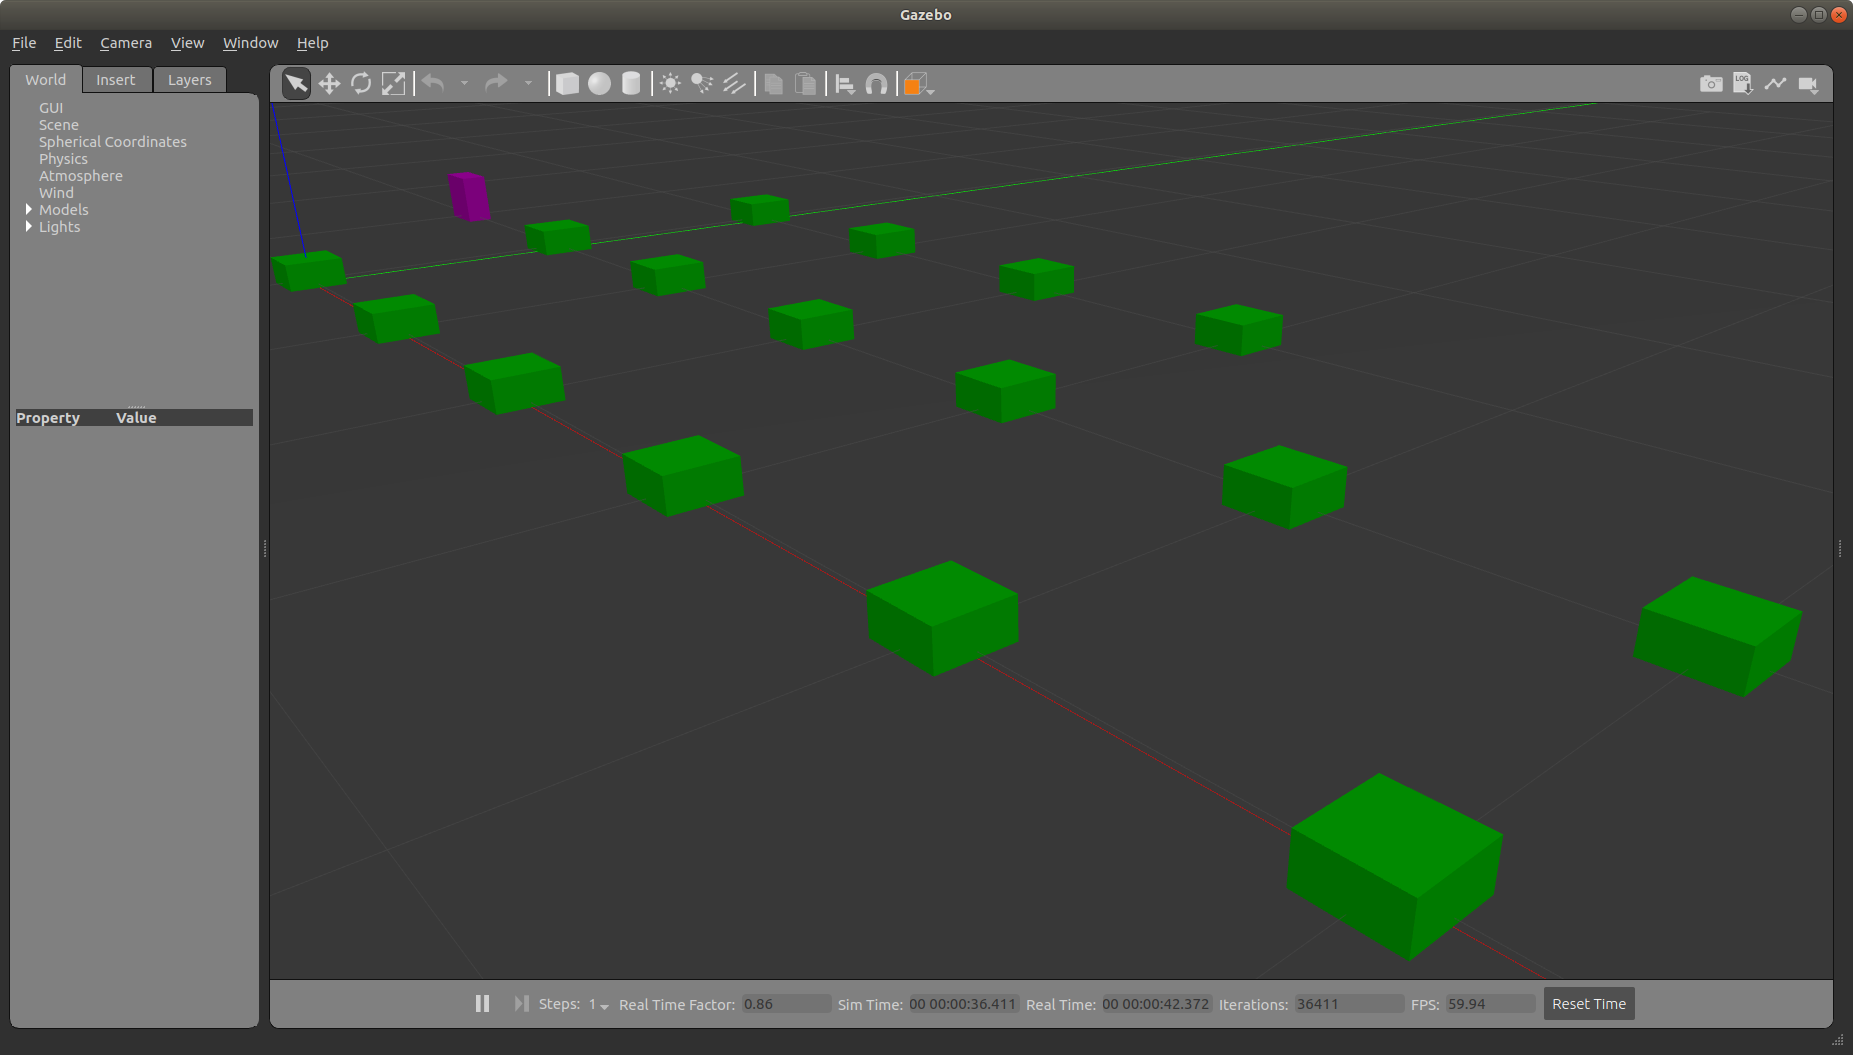
\includegraphics[width=.6\linewidth]{Afbeeldingen/dronegroep.png}\end{center}
	\caption{Groep van drones in de simulatie.}
	\label{fig:dronegroep}
\end{figure}

Wat hierin een uitdaging was, was het injecteren van de drone informatie in Gazebo en het vervolgens aansturen. Dit is gedaan via een SDF beschrijving \cite{sdf} die een plugin heeft die de drone voorziet van een motor zoals in het onderstaand voorbeeld te zien is. 

\begin{lstlisting}
<plugin name='DroneEngine' filename='libDroneEngine.so'>
	<DroneID>0</DroneID>
</plugin>
\end{lstlisting}

Deze motor kan vervolgens via een Ros service aangesproken worden. Zo kon er vanuit een aanroep in de console of het Ros programma RQT een drone verplaatst worden van positie. 

\paragraph{Directe communicatie}
Nu er drones in de simulatie mogelijk waren betekende dat er meshnetwerk componenten gekoppeld konden worden aan de drones in de simualtie.

Er is begonnen met het schrijven van een plugin die het netwerkcomponent representeerde in de simulatie. 
Vervolgens konden deze op twee drones `aangesloten' worden om vervolgens deze met elkaar te laten communiceren.
Het communiceren was nog een simpele applicatie waarbij een component een 32 byte array naar de andere moest sturen waarop het andere component weer response moest geven.
Dit lukte al vrij snel waarop de volgende stap was het limiteren van de communicatie op basis van de onderlinge afstand.

Hiervoor is de draadloze communicatie simulator tot stand gekomen. 
Deze applicatie moet draaien om onderlinge communicatie mogelijk te maken omdat de netwerkcomponenten niet meer direct met elkaar mogen praten.
In deze simulator zijn regels gesteld of het op basis van afstand het toegestaan is om een bericht te versturen.
Een uitdaging hierin was het op de hoogte blijven van de locatie van een node. 
Er is besloten dat dit aan de hand van een Rostopic zou gebeuren zodat een drone als die zich verplaatst continue zijn nieuwe positie door kan geven.
Een netwerkcomponent kan op zijn beurt op dit topic aangeven op welke drone hij aangesloten zit en op welk topic hij berichten wil ontvangen. De werking hiervan kon getest worden door drones met een directe aansturing te verplaatsen.

\paragraph{Broadcast}
Met een fysieke NRF24 antenne is het mogelijk om op een kanaal een bericht te versturen naar iedere andere NRF24 antenne binnen bereik.
Zo komt er een bericht aan via een zogeheten broadcast. 
In een simulatie werkt dit niet omdat er niet iets alle kanten opgestuurd kan worden.
Daarom is er besloten een functie toe te voegen aan de draadloze communicatie simulator waarmee opgevraagd kan worden wie er binnen bereik is.
Zo kon er toch een implementatie gemaakt worden waar een broadcast uitgevoerd wordt.

\begin{lstlisting}
bool WirelessSignalSimulator::getNodesInRange(
drone_meshnetwork_simulation::AreaScan::Request &req,
drone_meshnetwork_simulation::AreaScan::Response &res )
{   
auto from = Network.find( req.id );
res.near.clear( ); //Clear the response before filling.
if ( from != Network.end( ) ) {
	for ( std::pair< uint8_t, Node * > other : Network ) {
		if ( other.first == from->first ) continue;  //Not interrested in ourself
		if ( !other.second->getOn( ) ) continue; //Ignore nodes that are turned off
		// using pythgoras in the function Vector3 to get the distance between the
		// nodes
		float distance =
		from->second->getPosition( ).Distance( other.second->getPosition( ) );
		if ( distance < maxComDistance ) {
		res.near.push_back( ( int )other.first );
		}
	}	
	return true;
} else {return false;}
}
\end{lstlisting} 
 
\paragraph{Gateway router verbinding}
Nu er een implementatie was in de simulatie waarmee eigenlijk alle mogelijkheden nagebootst konden worden die een fysieke antenne zou kunnen aanbieden, was het tijd om te beginnen aan het implementeren van de routeringstechniek die uit het onderzoek gekozen was.

Een eis was dat het netwerk altijd bestaat uit minimaal één gateway en nul tot 100 routers.
Een logische stap was dus het scheiden van de logica van het netwerkcomponent in een gateway en in een router.
Een andere eis van het netwerk stelt dat een router altijd direct of indirect verbinding moet hebben met een gateway.
De volgende implementatie stap die genomen is, was het registreren in een router of deze daadwerkelijk een verbinding heeft met een gateway.
Er is voor gekozen om een pessimistische implementatie te maken waarbij een router alleen mag claimen dat hij een verbinding heeft met een gateway op het moment dat hij een bericht ontvangt van de gateway die voor hem geadresseerd is.
Deze berichten worden onderling uitgewisseld via een heartbeat. 

\begin{figure}[H]
	\begin{center}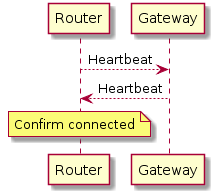
\includegraphics[width=0.2\linewidth]{Afbeeldingen/heartbeat.png}\end{center}
	\caption{Communicatie voor bevestiging verbinding.}
	\label{fig:bevestigingverbinding}
\end{figure}
\paragraph{Verbinding router naar een gateway}
Na het implementeren van een heartbeat voor een enkele router binnen bereik was de volgende stap om een heartbeat te implementeren voor een router buiten bereik het bereik van een gateway. Dit hield eigenlijk in dat er een implementatie moest komen voor het doorsturen van berichten. Er is eerst simpel begonnen met twee routers en een gateway. Het eerste deel van de route was het gemakkelijkste de gateway had namelijk altijd hetzelfde adres namelijk 0. Daarom kon er vrij snel al een implementatie gemaakt worden. In de applicatie, als de tussen node een bericht ontving voor 0 moet deze doorgegeven moest worden aan de gateway. De weg terug wordt nu complexer voor de gateway hij kan namelijk niet simpelweg het bericht terug sturen want dat is buiten het bereik.
\paragraph{Routeringstechniek}
Er moet dus een routeringstechniek gemaakt worden om bij de node te komen.
In het geval van de gateway is er de volgende kennis aanwezig:
\begin{itemize}
	\item Er bestaat een router met ID 2 buiten bereik
	\item De router met ID 1 die heeft direct of indirect een connectie met die router
\end{itemize}

Met die kennis is er de theorie dat als het bericht dat naar router ID 2 gestuurd moet worden aan router ID 1 gegeven wordt dat deze dan wel weet hoe het bij router 2 moet aankomen.
Deze theorie wordt toegepast in het lightweight mobile routing protocol \cite{LMR}.
Aan het nu abstracte netwerkcomponent is een routeringstabel toegevoegd waar in opgeslagen worden welke routers een directe verbinding hebben en bij elke van die routers wordt bijgehouden met welke routers zij weer een verbinding hebben.

\begin{figure}[H]
	\begin{center}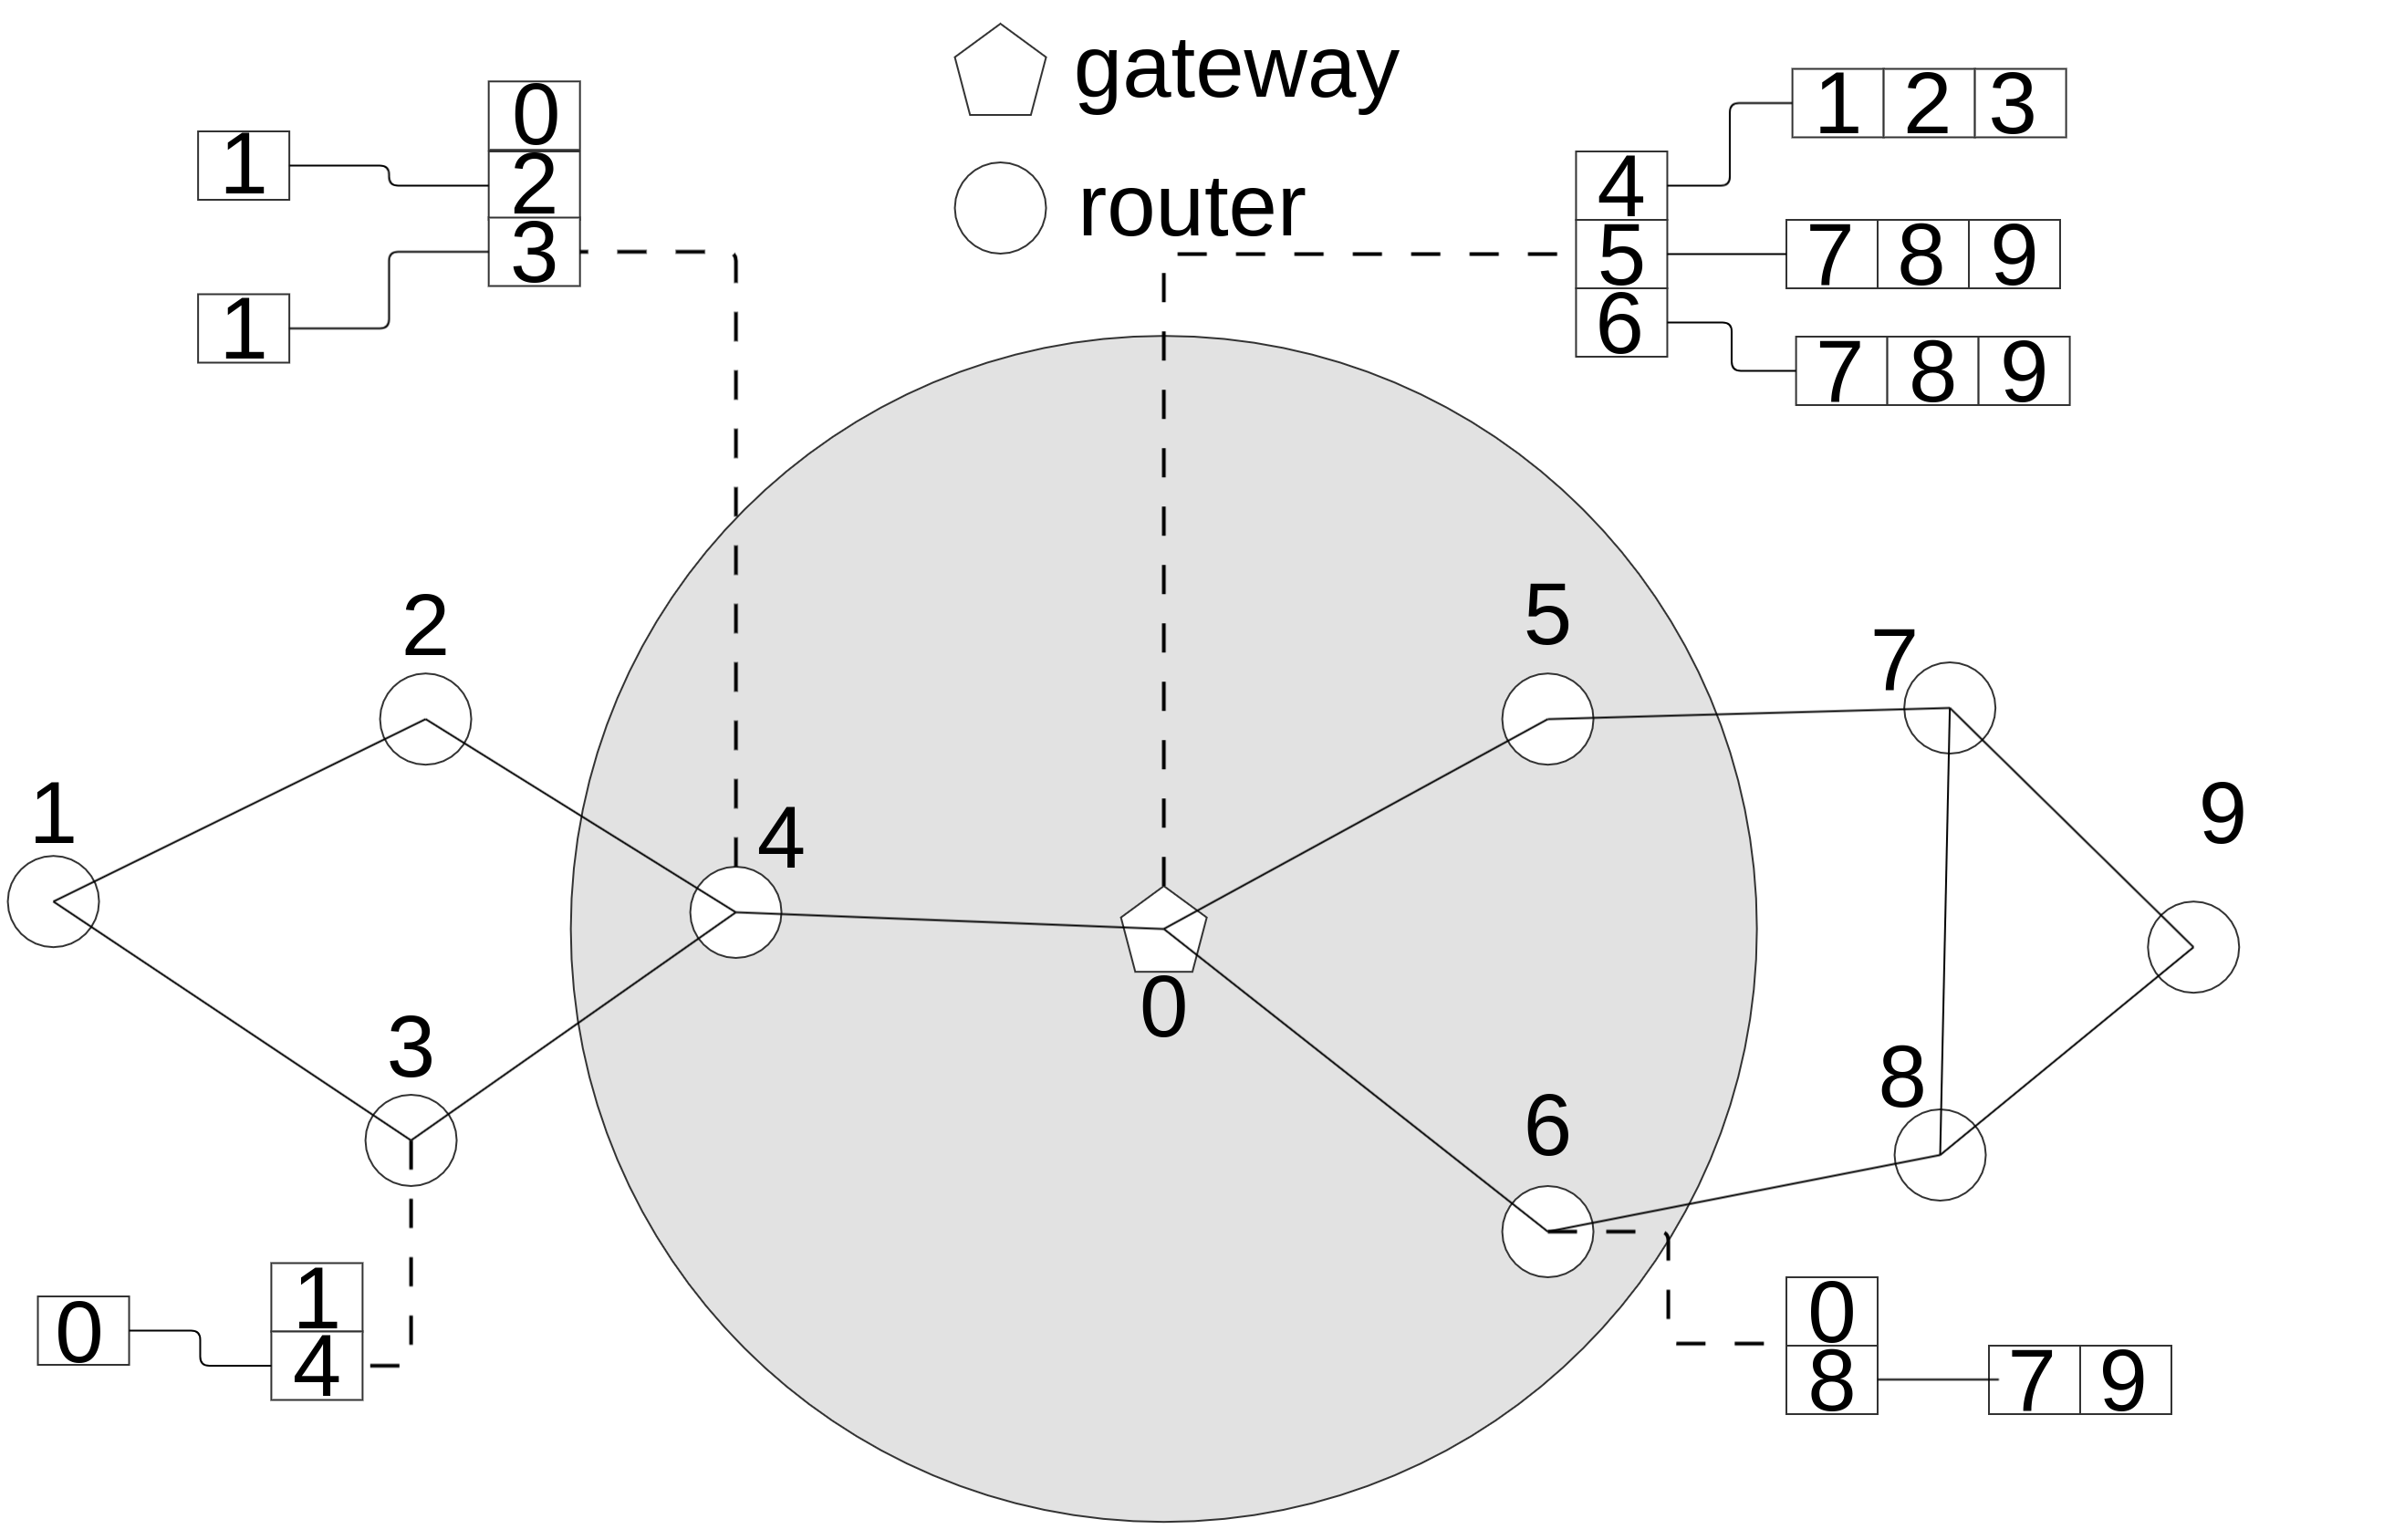
\includegraphics[width=0.6\linewidth]{Afbeeldingen/uitlegtabel.png}\end{center}
	\caption{Toelichting routeringstabel.}
	\label{fig:routeringstabel}
\end{figure}

In \autoref{fig:routeringstabel} wordt geïllustreerd hoe de routeringstabellen van de gateway en verschillende routers er uitzien.
Een nadeel van de huidige implementatie is dat er geen rekening wordt gehouden met het kortste pad door het netwerk.
Als in \autoref{fig:routeringstabel} bijvoorbeeld de gateway een bericht wil versturen naar router nummer 8 zal dit gebeuren via de weg 0-5-7-8 in plaats van de kortste weg 0-6-8. Dit komt omdat er nu eerst gekeken wordt of het bericht voor de geadresseerde een direct aangesloten punt is, als dat niet zo is worden de tabellen van de indirecte punten nagelopen. Omdat die op numerieke volgorde de tabellen van externe punten nazoekt zal de tabel van punt 5 als eerste een routepunt geven.

Wat ook opvalt aan de techniek is dat een router altijd op een manier een route weet naar een gateway toe. Dit maakt het dus altijd mogelijk om de gateway als punt aan te houden als er een communicatieweg gevonden moet worden naar een onbekend punt met als regel dat een bericht niet in de richting teruggestuurd mag worden waar die een vorige stap ook was.

Als laatste punt over LMR moet benoemd worden dat het netwerk zich event driven onderhoudt.
Dit houdt in dat er alleen informatie wordt rondgestuurd over nieuwe of verbroken verbindingen op het moment dat er een wijziging optreedt in het netwerk. 
Volgens de LMR techniek wordt een verbroken verbinding pas gedetecteerd op het moment dat vinden van een pad naar een aangesloten buur niet lukt.
Omdat de opdracht was dat het netwerk snel moet doorhebben dat een verbinding verloren is, is er toegevoegd dat elk punt periodiek de verbinding van direct aangesloten punten naloopt. 
Deze routeringstechniek is voorzien van unittesten die testen of de routes daadwerkelijk gevonden worden en de tabellen juist worden bijgehouden.
Een voorbeeld van een test is hieronder te zien.
\begin{lstlisting}
TEST( TestSuiteHybridLMRoutingProtocol, findRouteToGrandChild )
{
	HybridLMRoutingProtocol CTT;
	CTT.OtherCanCommunicateWithNode( 1, 4 );
	CTT.OtherCanCommunicateWithNode( 2, 5 );
	CTT.OtherCanCommunicateWithNode( 3, 5 );

	EXPECT_TRUE( CTT.getDirectionToNode( 5 ) == 2 );
}
\end{lstlisting}

\paragraph{Berichten}
Binnen het netwerk worden compacte berichten gebruikt die een vaste volgorde in een 32 byte array hebben.
Deze worden per byte in de array geplaatst en aan de andere kan er weer uitgehaald.
De code die hier hoofdzakelijk voor gebruikt wordt zijn twee functies die als volgt gaan:
\begin{lstlisting}
 void Message::CopyToCharArray( uint8_t *value, uint16_t size, uint8_t *arr,
uint16_t start )
{
for ( uint16_t i = 0; i < size; i++ ) {
	arr[i + start] = value[i];
	}
}

void Message::CopyFromCharArray( uint8_t *value, uint16_t size,
const uint8_t *arr, uint16_t start )
{
for ( uint16_t i = 0; i < size; i++ ) {
	value[i] = arr[i + start];
	}
}
\end{lstlisting}
In de eerst functie wordt een waarde per byte gekopieerd naar een array van byte.
De tweede functie doet juist het omgekeerde.
Een belangrijke voorwaarde is dat de programmeur precies weet hoe groot het data type is en op welke plek de waarde in een array staat. 


Om te zorgen dat deze berichten juist in een array gezet worden en er ook weer juist uitgehaald worden is elke type bericht voorzien een meerdere unittesten.
Naast de standaard unit testen worden ook bijzondere locaties getest zoals de locatie van Lelystad airport waar de landingsbaan onder zee niveau ligt.
Dit te zien in de volgende test:
\begin{lstlisting}
TEST( TestMessages, locationLelystadAirportMessageToPayload )
{
float lat = 52.455702;
float lon = 5.519210;
int16_t hei = -5;
uint32_t time = 1557435698;

LocationMessage amsg( 66, 55, 44, 33, lat, lon, hei, time );
uint8_t buffer[MAX_PAYLOAD];
amsg.toPayload( buffer );

LocationMessage msg( buffer );

EXPECT_EQ( LOCATION, msg.getMessageType( ) );
EXPECT_EQ( lat, msg.getLatitude( ) );
EXPECT_EQ( lon, msg.getLongitude( ) );
EXPECT_EQ( hei, msg.getHeight( ) );
EXPECT_EQ( time, msg.gettimeSincePosix( ) );
}
\end{lstlisting}

\paragraph{Drone aansturing}
Nu er communicatie mogelijk is tussen de netwerkcomponenten, en deze in staat zijn correct te kunnen detecteren of er een verbinding naar een gateway mogelijk is, kunnen de componenten aangesloten worden op de interface van de drone voor aansturing.
Omdat de abstracte drone niet via een enkele interface aangestuurd kan worden is gebruik gemaakt van een adapter \cite{adapter} tussen het netwerkcomponent en de drone. 
De adapter is te zien in \autoref{fig:adapter}.

\begin{figure}[H]
	\begin{center}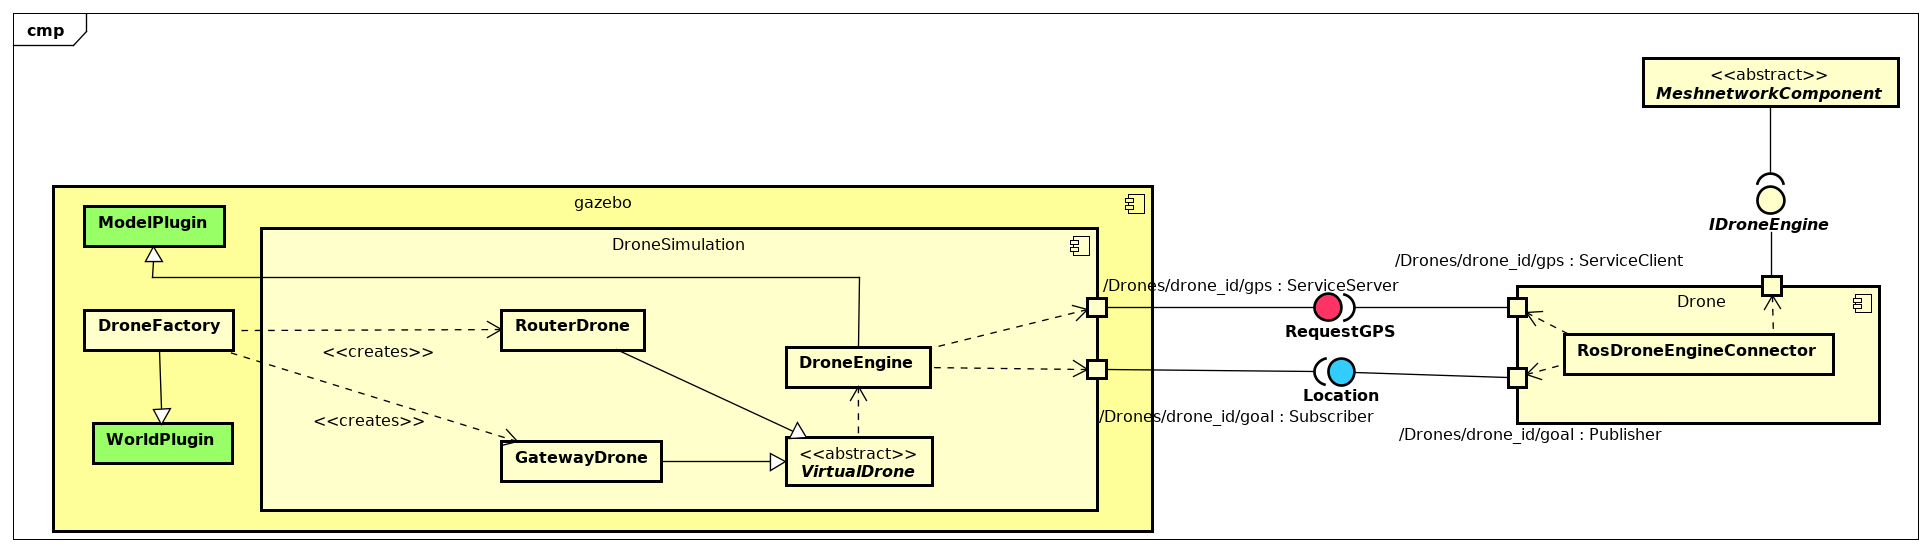
\includegraphics[width=1\linewidth]{Afbeeldingen/RosEngineAdapater.png}\end{center}
	\caption{Uitwerking adapter tussen de DroneEninge en het MeshnetwerkComponent.}
	\label{fig:adapter}
\end{figure}

Ook hier is weer simpel begonnen door, het eerst mogelijk te maken door met het ontvangen van een bericht op het netwerkcomponent een doel te sturen naar een dronemotor. Vervolgens kon er getest worden of dit werkte door zelf een bericht op te stellen en dit direct naar de antenne te sturen van de netwerkmodule. 
Bij het ontvangen van het bericht zal de drone zich verplaatsen naar de locatie die opgegeven is.

\paragraph{Dronemanager}
Omdat er nog geen manier was om op een simpele manier berichten het netwerk in te kunnen sturen is de dronemanager ontwikkeld. Deze applicatie start een Rosservice die communiceert op een Rostopic waar alle gateways naar luisteren. Omdat er alleen interesse is naar het versturen van locaties naar drones kan ook alleen dit gepubliceerd worden op het topic.
\begin{figure}[H]
	\begin{center}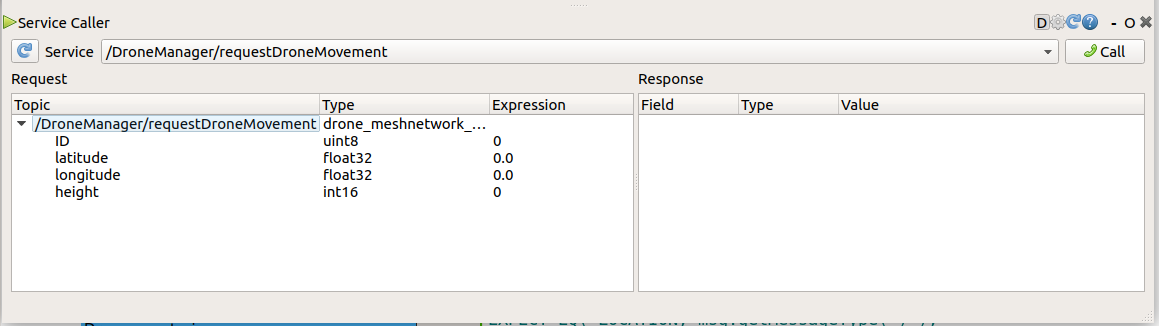
\includegraphics[width=1\linewidth]{Afbeeldingen/LocationMessageRQT.png}\end{center}
	\caption{Het versturen van een verplaatsingsverzoek via de dronemanager.}
	\label{fig:serviccaller}
\end{figure}

Zodra een gateway een nieuw bericht ontvangt op het topic maakt hij hier een bericht van die het netwerk ingestuurd wordt met een verzoek voor verplaatsing. Op deze manier kon ook makelijker getest worden of de drone aansturing goed werkte en of een punt ver weg in het netwerk daadwerkelijk in staat was berichten van een gateway te ontvangen.

\paragraph{Protocol bij een verloren verbinding met de gateway}
De opdracht stelt dat drones zich moeten verplaatsen bij een verloren verbinding naar een alternatieve locatie om zo te proberen de verbinding te herstellen. 
Hier was de eerste stap om eerst te ontdekken of een netwerkmodule alleen is of dat er nog andere punten in de buurt zijn die ook een verbinding verloren zijn. 
Hiervoor kon de broadcast functie goed gebruikt worden.
 De meeste simpele implementatie kon vervolgens gemaakt worden voor de drone die in zijn eentje de verbinding met de gateway verloren is. 
Na overleg met Alten is besloten dat het voor nu voldoende was als de drone eerst terug vliegt naar het punt dat verloren is gegaan om daar te zoeken naar een nieuwe verbinding met de gateway.
Op het moment dat daar nog steeds geen verbinding gevonden is moet de drone terug keren naar de locatie waar de gateway staat.   

Op het moment dat er groep is die verloren gaat moet er een overleg gepleegd worden tussen de drones, het heeft immers geen zin om allemaal naar een zelfde locatie te bewegen of om twee werkende netwerkmodules op een plek te parkeren. 
Er is nu geïmplementeerd dat elke drone berekend wat zijn afstand is tot de gateway, de drone met de grootste afstand die wil verplaatsen naar een plek waar nog geen andere drone staat zal een beweging uitvoeren.  

Een demonstratie hiervan is te zien in de video's van bijlage \ref{sec:videos-simulatie-netwerkherstel-door-drone-verplaatsing}.
   
\paragraph{Meerdere gateways in een netwerk}
Een wens van Alten is de mogelijkheid om meerdere drones te gebruiken in een netwerk. 
Hiervoor is logica toegevoegd aan de routers dat er een voorkeur voor een gateway bestaat.
Op het moment dat een router een bericht krijgt van een ander punt in het netwerk die minder hops tot aan een gateway heeft dan neemt de router het id over van de voorkeur gateway van dat punt. 

Een video waar de werking van twee gateways in het netwerk gedemonstreerd wordt is te vinden in bijlage  \ref{sec:gatewaywisselmp4}

\paragraph{Fysiek prototype router}
Na de oplevering van de 80 procent versie is er gewerkt aan de oplevering van een fysieke netwerkmodule.
Hiervoor was de makkelijkste stap om de router software draaiende te krijgen op de raspberry.
Dit omdat alleen het virtuele NRF24 component vervangen hoefde te worden voor een fysieke.
In eerste instantie verliep dit goed, vooraf waren er al ontwerpen gemaakt op basis van de beschikbare NRF24 libary \cite{nrf24git}.

Wat een tegenvaller was, was dat ik vergeten was dat er een Vector3 gebruikt werd uit de libary die meegeleverd wordt met Gazebo.
Omdat er in de software alleen de Vector3 een afhankelijk heeft naar de libary is er besloten de Vector3 zelf te implementeren in een template class.
Na het implementeren van deze template class kon er een router programma gecompileerd worden voor de Raspberry Pi.

\begin{figure}[H]
	\begin{center}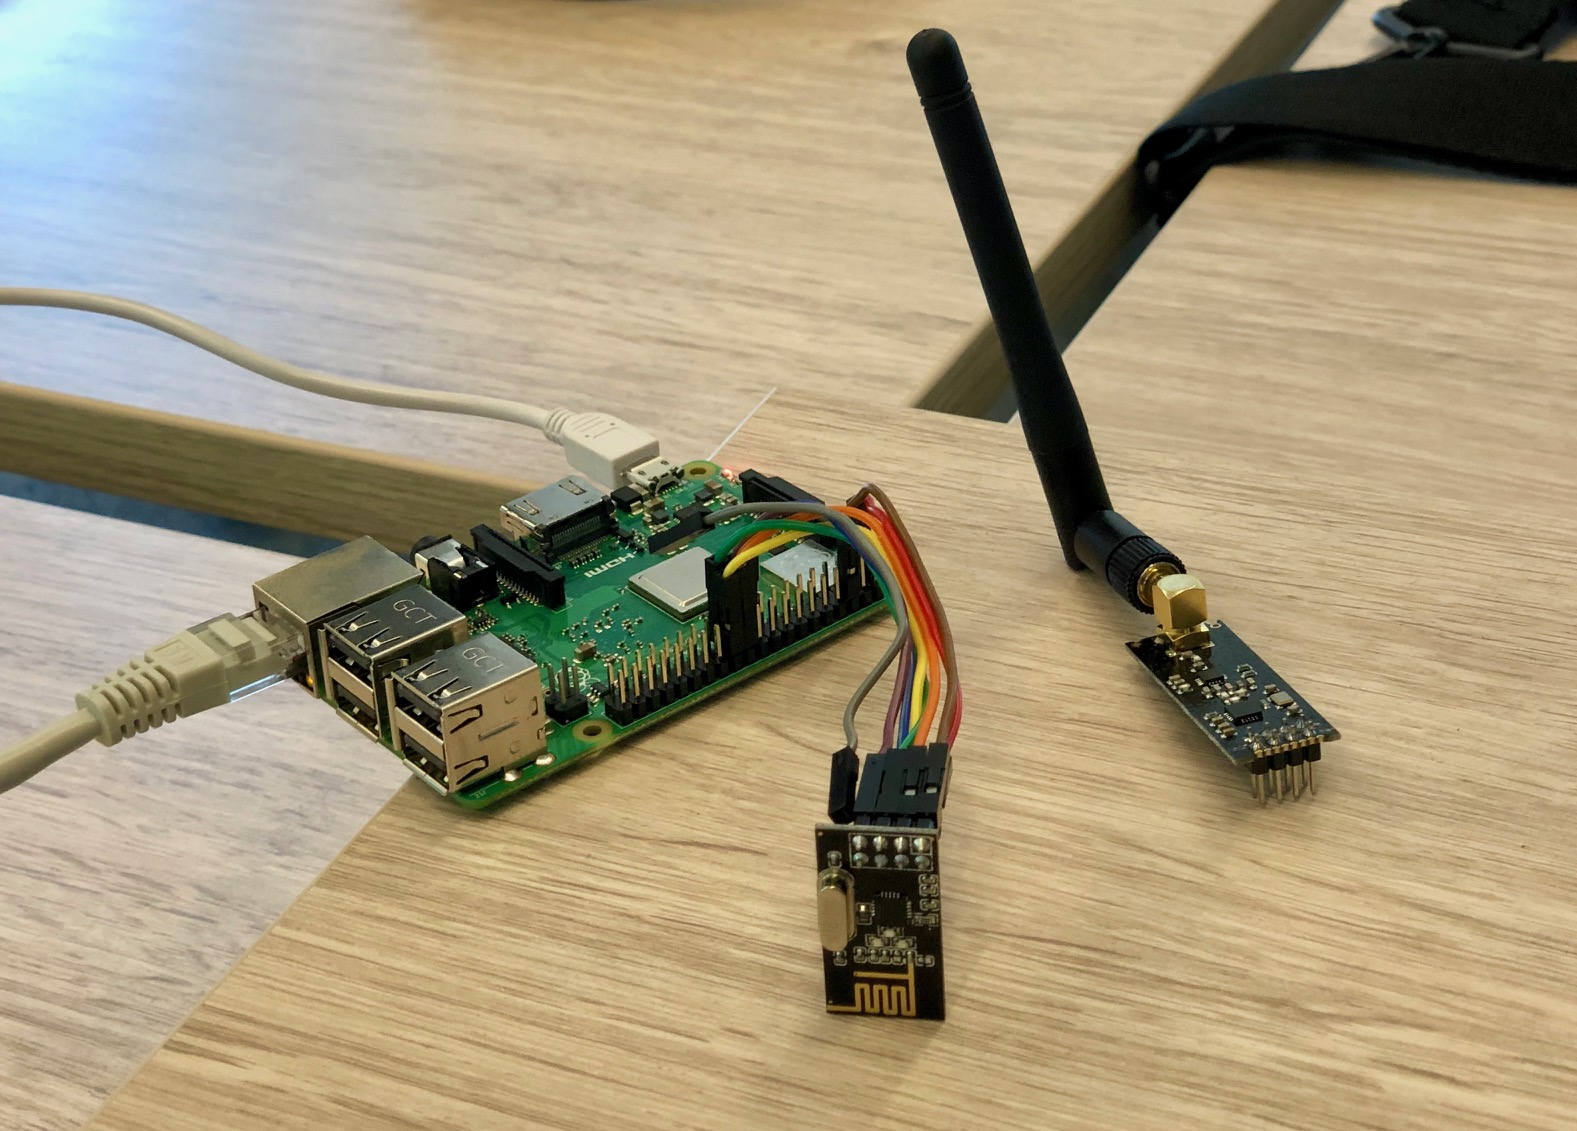
\includegraphics[width=.7\linewidth]{Afbeeldingen/raspberryOpKantoor.jpg}\end{center}
	\caption{Raspberry aangesloten op de antenne voor korte afstand.}
	\label{fig:raspopkantoor}
\end{figure}

Door twee Raspberry Pi's op het netwerk aan te sluiten van Alten (\autoref{fig:raspopkantoor}) konden ze via een ssh verbinding gestart worden om met elkaar te communiceren wat het eerst contact via de fysieke NRF opleverde te zien in bijlage \ref{sec:eerstecontactmp4}.

\paragraph{Fysiek prototype gateway}

Tenslotte was er nog net tijd voor een laatste implementatie die de oplevering compleet zou maken naar wat beloofd is in het begin van het project.
Kort overleg gaf de goedkeuring om zonder uitgebreid onderzoek een C++ libary te pakken voor de internetgateway.
Deze goedkeuring was gebaseerd op het feit dat het toch om een prototype ging en het gewoon heel cool zou zijn om alles op te kunnen leveren.
Na kort zoekwerk op het internet kwam Pistache \cite{pisrest} naar voren vanwege het gemak voor het opzetten van een REST framework.

Wat een mooi moment was voor mij als programmeur was dat ik de service eerst ontwikkeld heb voor de gesimuleerde gateway.
Vervolgens heb ik de Pistache libary geïnstalleerd op de Raspberry Pi en kon daar zo dezelfde software draaien als in de simulatie.
Dit bewees voor mij het nut van de simulatie als ontwikkelaar omdat de simulatie mij dus de mogelijkheid biedt software te ontwikkelen op mijn pc voor mijn pc.
Vervolgens kan ik deze software op de Raspberry Pi zetten en dezelfde code compileren.

Een video met audio is te vinden in bijlage \ref{sec:fysieke-router-en-dronemp4} waar de gateway getoond wordt in samenspel met een router.

\chapter{Resultaten}\label{sec:resultaten}

%Inhoudelijk, wat heb je opgeleverd, met welke kwaliteit? Was dit ook volgens plan? Ben je afgeweken en zo
%ja waarom?
%(Deze laatste drie kunnen ook geïntegreerd worden)
In de dit hoofdstuk worden de opgeleverde producten behandeld en beoordeeld op hun kwaliteit.

\section{Plan van aanpak}\label{sec:plan-van-aanpak}
Het eerste product die is opgeleverd was het plan van aanpak.
Het product kreeg zijn echte waarde na de feedback op het conceptplan.

Het eerste plan was nog niet concreet genoeg in wat opgeleverd zou ging worden. 
Dit was dan ook in grote lijnen wat de feedback was vanuit de begeleiders van school.

Na het verwerken van de feedback was het plan veel gerichter in wat opgeleverd zou moeten worden.
Het plan dat er nu ligt zou uitgevoerd kunnen worden door elke ICT'er met de juiste vaardigheden.
De kwaliteitseis die ik gesteld heb aan het plan van aanpak was dat het moest omschrijven wat het plan van de student is en dat het voldoet aan het feedbackformulier projectplan van het \citeauthor{HANfeed} \citeyear{HANfeed}. Deze kwaliteitseisen zijn voldaan wat dus betekend dat het op papier voldoet aan alle kwaliteit.

Wat in mijn ogen nog beter bewijst dat het plan van aanpak een document van kwaliteit is, is dat ik gedurende het project regelmatig het plan erbij heb gepakt om beslissingen op te baseren en kwaliteit van andere producten mee te meten.

\section{Broncode}\label{sec:broncode}
De code geschreven voor dit project heeft veel aandacht van mij gekregen. 
Er heeft veel moeite gezeten in het gebruik van Doxygen om dit volledig compleet te houden.
Als resultaat geeft dit dan een compleet resultaat bij het generen van de documentatie. 

Daarnaast wat wel is uitgevoerd maar naar mijn mening te weinig is toegepast is het gebruiken van unittesten.
Dit is weinig gebruikt omdat veel code een communicatie uitvoert naar een andere netwerkcomponent.
Er kunnen wel unittesten voor geschreven worden maar het opzetten van een basis voor zulke testen kost veel tijd.
Toch zou ik Alten wel adviseren als ze dit project voortzetten om hier in te investeren.
Het schrijven van een routeringstechniek is een complex proces die snel problemen kan geven.
Het breder toepassen van unittesten zou de kwaliteit van het meshnetwerk zeker ten goede komen. 

De componenten zijn op elkaar aangesloten door interfaces aan elkaar aan te bieden.
Dit is gedaan om meerdere redenen. 
Door elkaar interfaces aan te bieden bewaakt een component zijn toegang tot de publieke functies.
Daarnaast bieden de interfaces een potentie voor het schrijven van testen omdat deze gemockt kunnen worden.  

Wat jammer is maar niet mogelijk was in het project was dat er geen buildserver beschikbaar was waar een geavanceerde codeanalyse tool aan gekoppeld zit zoals coverity of sonarqube. Wel is er in het project gebruik gemaakt van de statische codechecker CPPcheck. Hoewel het geen maatstaaf is hier nul meldingen op te krijgen in verband met false positives. 
Toch is bij elke melding die CPPcheck heeft gegeven afgehandeld ofwel door het aanpassen van code of door het bewust onderdrukken van de functie. Zo zijn er op dit moment alleen meldingen onderdrukt over ongebruikte debugging functies of een het gedeelte waar een float wordt opgeknipt in bytes.
  
\section{Onderzoeksrapport}\label{sec:onderzoeksrapport}

Het onderzoeksverslag is een verslag die naar mijn mening inhoudelijk niet voldoende gespreide aandacht heeft gekregen. Hoewel het misschien de onderzoeksvraag beantwoord is er duidelijk te merken dat het literatuur onderzoek naar de te gebruiken hardware en simulatiesoftware veel meer tijd heeft gekregen dan de rest van het document.

De hoofdvraag gesteld in het onderzoek is relevant omdat het helpt met het uitvoeren met de specifieke opdracht.
De deelvragen daarentegen zijn niet allemaal even sterk uitgewerkt. 
Zo is er de vraag wat nodig is om een abstracte drone te representeren. 
Hier had ik veel onderzoek naar kunnen doen maar dit heeft geen meerwaarde. 
Een kort overleg voldoet in dit onderwerp ook waarin besproken is van wat moet de gesimuleerde drone allemaal kunnen.

Op zich is dit gezien de beschikbare tijd een prima keuze maar het haalt de kwaliteit van het onderzoek wel naar beneden.

Wat goed is gedaan in het onderzoek is het gebruik van bronnen, zo zijn ze voornamelijk gebaseerd op wetenschappelijke artikelen en zijn ze ruim aanwezig.

Verder merkte ik dat het fijn is voor het bedrijf dat de onderzoeksmethode geleerd op de HAN nog toegelicht is aangezien niet iedereen hiermee bekend is. Ook het toelichten hoe onderzoek op de HAN werkt is goed onderbouwd en toegelicht.
  


\section{Simulatiesoftware}\label{sec:simulatiesoftware}
Tegen het einde van het project werd de simulatiesoftware opgeleverd. 
Dit was het product waar de meeste focus en ontwikkeling in heeft gezeten.
Dit was initieel niet het plan omdat er meer focus op het hardware prototype zou liggen.
Gedurende het project werd de urgentie van de simulatiesoftware steeds duidelijker.

Door het gebrek aan voldoende hardware kon er niet goed getest worden hoe het netwerk zich zou gedragen bij een hoog aantal nodes.
Daarom is er gekozen om de simulatie een hogere prioriteit te geven zodra de gesimuleerde communicatie realistisch genoeg was.

Een tegenvaller van de simulatie in Gazebo was dat voor het simuleren van 100 drones en dit visueel te maken een computer met een dedicated GPU nodig is. Dit was vooraf niet verwacht omdat de drones in de simulatie alleen maar vliegende blokjes zijn. 

Het opgeleverde product voldoet wel aan de wens van Alten. Alten wil namelijk verdeelalgoritmes kunnen testen waarbij de drones op een realistische wijze worden aangestuurd, en dat is opgeleverd.  Verder is de simulatie voorzien van voldoende documentatie.  

\section{Hardwareprototype}\label{sec:hardwareprototype}
Het huidige hardware prototype staat nog echt in de kinderschoenen.
Hoewel het routeringsprotocol die gebruikt wordt in het prototype zichzelf bewezen heeft in de simulatie is deze summier getest in de fysieke wereld.
Daarom kan er onvoldoende garantie gegeven worden op het gedrag van het prototype.
Dankzij de opzet van de code kan er wel eerst getest worden in de simulatie waarna het vervolgens mogelijk is om de code direct te draaien op de prototype.
Dit zal de doorontwikkeling aanzienlijk versnellen voor het prototype.



\section{Software requirements specificatie}\label{sec:software-requirements-specificatie}
Voordat er een goed design kan komen is het zaak dat er requirements opgesteld worden.
Dit heb is gedaan door het opstellen een software requirements specificatie.  
Deze heb is opgesteld aan de hand van gesprekken met de opdrachtgever Alten.
In deze gesprekken zijn de gesprekstechnieken ANNA (altijd navragen nooit aannemen) en LSD (luisteren samenvatten doorvragen) toegepast zoals dit geleerd is in de professional skills lessen.  
Vervolgens zijn de requirements opgedeeld in functionele requirements en niet functionele requirements. 
De functionele requirements zijn door de MoSCoW methode toe te passen geprioriteerd.
De niet functionele requirements zijn vervolgens verdeeld in categorieën uit FURPS. 

\section{Software design document}\label{sec:software-design-document}
Het software design document is zo compleet mogelijk opgeleverd.
Er gekozen om niet per subcomponent het design te behandelen maar dit te doen per package.
Deze keuze is gemaakt omdat de componenten die in elke package zitten niet zonder elkaar behandeld kunnen worden.
Zo is bijvoorbeeld de virtuele NRF24 een component die alleen communiceert via het component die draadloze communicatie afhandelt.
Dit komt door het gebruik van Ros.
Omdat er door het toepassen van Ros een aantal subcomponenten van het systeem als aparte applicatie draaien.

Verder als het design document tegen de kwaliteitseisen die in het plan van aanpak zijn gesteld wordt gehouden dan voldoe deze aan de gestelde eisen.
Het document komt overeen met de code en alle relevante ontwerpen zijn ruimschoots vastgelegd.
Wat afwijkt in het proces ten opzicht van het plan is de stap waar het domeinmodel wordt omgezet tot class diagrammen. 
Er is gekozen om gebruik te maken component diagrammen die de samenhang van de software overzichtelijker maken dan een class diagram. 


\chapter{Evaluatie}\label{sec:evaluatie}
%Evaluatie/ Reflectie / Situaties (STARR)
%Inzichten!
%Inzichten mbt proces, producten en resultaten, èn het eigen functioneren. middels een methode als STARR.
%Die methode moet dan wel goed toegepast worden.
In dit hoofdstuk worden situaties behandeld die zich tijdens de afstuderen hebben voorgedaan. 
Hiervoor wordt de STARR (Situatie, Taak, Actie, Resultaat, Reflectie) methode toegepast. 

\section{80\% versie}\label{sec:altijd-navragen-nooit-aannemen}
Het is zo verteld door de professional skills leraren en toch heb ik in dit project de fout gemaakt om iets aan te nemen.
Deze situatie beschrijft hoe dit project flink is beïnvloed omdat ik een aanname had gedaan ten opzichte van de 80\% versie.

Tijdens de eerste fase van het project moet elke student een plan van aanpak schrijven. Hierin is een belangrijk stuk de planning. Tijdens het plannen van het project heb ik de fout gemaakt om zo te plannen dat er bij een 80\% versie het project ook 80\% voltooid zou zijn. Dit leek ook allemaal logisch tot er de evaluatie kwam van een plan onder begeleiding van Jorg Visch. Pas toen kwam ik erachter dat het beter zou zijn voor de kans van slagen dat het project tijdens de 80\% versie tenminste alle elementen al zou bevatten om te kunnen slagen. 
Op dat moment was de planning hier nog niet naar terwijl dit plan al aardig strak gepland was.

Eerst had ik nog idee dat als ik iets harder zou werken en voor zou gaan lopen op de planning dat ik nog steeds een 80\% versie zou kunnen opleveren die zou voldoen aan de wensen vanuit school. Na drie weken in het project werd het duidelijk dat dit niet genoeg zou zijn. Er moest een geschoven worden binnen de planning om het toch allemaal op orde te krijgen.

Tijdens het project was er ook een terugkomdag op school, hier sprak ik met andere studenten onder andere over het 80\% inlevermoment. Zij vertelde mij dat ze al wel vroeg tijdens het schrijven van het plan van aanpak wisten dat ze zo moesten plannen dat er bij 80\% een project moest staan die waardig is voor slagen.

Hieruit leerde ik dat hoe logisch iets ook klinkt dat ik nooit is zomaar moet aannemen. Het effect van de verkeerde aanname is groot geweest op mijn project terwijl die eigenlijk makkelijk voorkomen had kunnen worden. Ik had in plaats van de aanname een mail naar mijn schoolbegeleider moeten sturen met de vraag naar wat hij verwacht van de inlevermomenten.  
  


\section{Afstudeereiland}
Deze situatie kaart ik aan omdat ik het afstuderen als eenzaam heb ervaren.
Natuurlijk zijn er de begeleiders en collega's waaronder ook oud HAN studenten aanwezig die zorgen voor de nodige gezelligheid en zijn ze allemaal bereid om mij te helpen.
Daarnaast is het afstudeerproject ook een proeve die een student alleen moet doorlopen.
Toch heb ik mij op een aantal momenten eenzaam gevoeld gedurende het project vandaar dat ik het afstudeereiland noem.

Dit eiland komt vooral omdat de afstudeeropdracht geen directe impact heeft op de productontwikkeling binnen het bedrijf. Hierdoor voelen collega's zich ook niet verplicht om zich te verdiepen in het werk wat ik uitvoer. 

Als student van de HAN informatica is dit voor mij voor het eerst dat ik een project alleen uitvoer. 
Zo werden alle voorgaande projecten met ongeveer 5 mensen uitgevoerd met zelf een uitzondering in het World of Robots project die met 17 personen werd gedaan.
Een project van 20 weken alleen is dus even wennen.
Het heeft mij de waarde van samenwerken aan een project veel meer leren waarderen dan ik al deed. 

Het werken op een eiland brengt meerdere nadelen met zich mee.
Het eerste nadeel is dat het alleen werken ten kostte gaat van de kwaliteit van het product.
Omdat er geen dagelijks contact is zoals dat bijvoorbeeld is in een daily stand up loop je niet alleen een groot risico dat wanneer een project een verkeerde richting op gaat dat dit pas laat onderkent wordt. Maar zijn er ook geen hoog frequente checks op de technieken toegepast binnen de producten.

Een ander nadeel dat kan optreden maar door Alten is voorkomen is dat ik makkelijk buiten de organisatie kon gaan vallen.
Alten heeft dit voorkomen door mij overal actief bij te betrekken en mij dezelfde toegang te geven tot activiteiten die normale collega's ook hebben. Zo heb ik presentaties bijgewoond waar bijvoorbeeld een kijkje in de softwarekeuken werd gegeven van de gigant takeaway.com(thuisbezorgd.nl) maar heb ik ook met het hele team op de schaatsbaan in Enschede gestaan om te curlen. Dit was allemaal optioneel en kon ik mij zelf voor aanmelden.

Een les die ik hier uit leer is dat ik meer mijn best had moeten doen om collega's inhoudelijk te betrekken bij mijn afstuderen. Dat het afstuderen alleen uitgevoerd moet worden is een feit maar dit betekend nog niet dat het eenzaam hoeft te zijn.

Ik had collega's meer kunnen betrekken door presentaties te geven over inhoudelijke keuzes in het project. Dit zou hun de kans geven om gericht feedback te geven over mijn werk. Terugkijkend ben ik hier zelf niet proactief genoeg in geweest.

Als ik terugkijk naar wat ik nog meer had kunnen doen denk ik dat alleen maar zou kunnen adviseren aan toekomstige afstudeerders om te gaan werken aan afstudeeropdrachten die invloed hebben op het product van het bedrijf. Dit forceert het bedrijf om zich actief met de student bezig te houden omdat de impact van het resultaat groter is. 

\section{Presentatie oefening voor verdediging}
Om te oefenen voor de verdediging en mijn collega's inzicht te geven in mijn product heb ik een presentatie gehouden zoals ik dat zou doen tijdens mijn verdediging.
De presentatie is gehouden voor een publiek van negen engineers.
Om op de presentatie feedback te krijgen heb ik gebruik gemaakt van een feedbackformulier waar de focus lag op mijn presentatie skills.
Er was ruimte op het formulier om schriftelijk feedback te geven, en er kon met -, + of ++ een waardering gegeven worden.
Aan het einde van de presentatie konden er vakinhoudelijke vragen gesteld worden zoals dat bij de echte verdediging ook zou zijn..
\subsection{Feedback op de presentatie}
Als eerste wil ik de feedback ingevuld op het formulier behandelen die de kwaliteit van de presentatie behandeld.
De feedback is opgedeeld in structuur, inhoud, non-verbaal, spreekstijl, visueel en contact met publiek.
Elk stuk wordt hieronder apart behandeld.
\subsubsection{Structuur (-[0], +[4], ++[4], leeg[1]) }

In de feedback wordt aangegeven dat de opbouw goed is.
Een terugkerend punt die in de feedback staat is dat er niet genoeg aandacht wordt gegeven aan de probleemstelling.
\subsubsection{Inhoud (-[0], +[3], ++[4], leeg[2]) }
Ook de feedback over de inhoud was positief.
Het publiek was tevreden over mijn kennis over de zaken en het verhaal werd duidelijk verteld.
Ze vonden de reflectie over het project een leuke toevoeging 

Punten uit de feedback zijn dat ik niet moet twijfelen over wat ik moet uitleggen. 
Ik bepaal van te voren wat ik wil toelichten.
Tijdens de presentatie gebruik het woord ``we'' op het moment dat ik beslissingen toelicht.
Als feedback wordt aangegeven dat ik niet we maar ik moet gebruiken, het is wellicht met Alten overlegd maar het is mijn project.
\subsubsection{Non-verbaal (-[0], +[6], ++[1], leeg[2])}
Ook hierover waren de feedbackgevers positief. Er wordt aangegeven dat ik autoriteit uitstraal, zeker overkom en een rustige sfeer heb. 
Leerpunten die gegeven worden zijn dat ik moet letten waar ik naartoe kijk dus niet te veel naar hetzelfde persoon of het bord.
\subsubsection{Spreekstijl (-[0], +[3], ++[6], leeg[0])}
Over de spreekstijl waren mijn collega's heel enthousiast.
De rust die ik tijdens de presentatie bewaarde waren ze niet gewend van stagiaires.
Ik praatte duidelijk en articuleerde goed.
Wel moest ik oppassen dat de rust die ik had niet ten kostte zou gaan van mijn enthousiasme. 

\subsubsection{Visueel (-[1], +[6], ++[0], leeg[2])}
Het visuele gedeelte was een minder sterk stuk de presentatie. 
Zo waren bepaalde figuren zoals het domeinmodel onleesbaar voor het publiek.
De demo filmpjes hadden last van het zonlicht waardoor het niet goed zichtbaar was voor iedereen.
Een collega vond ook dat ik de presentatie te veel als leidraad gebruikte en heeft daarom een - gegeven.

Waar de collega's positief over waren was een zelfbedachte techniek die ik gebruikt heb in mijn presentatie.

\begin{figure}[H]%
	\centering
	\subfloat[Slide waar het pad geintroduceerd wordt.]{{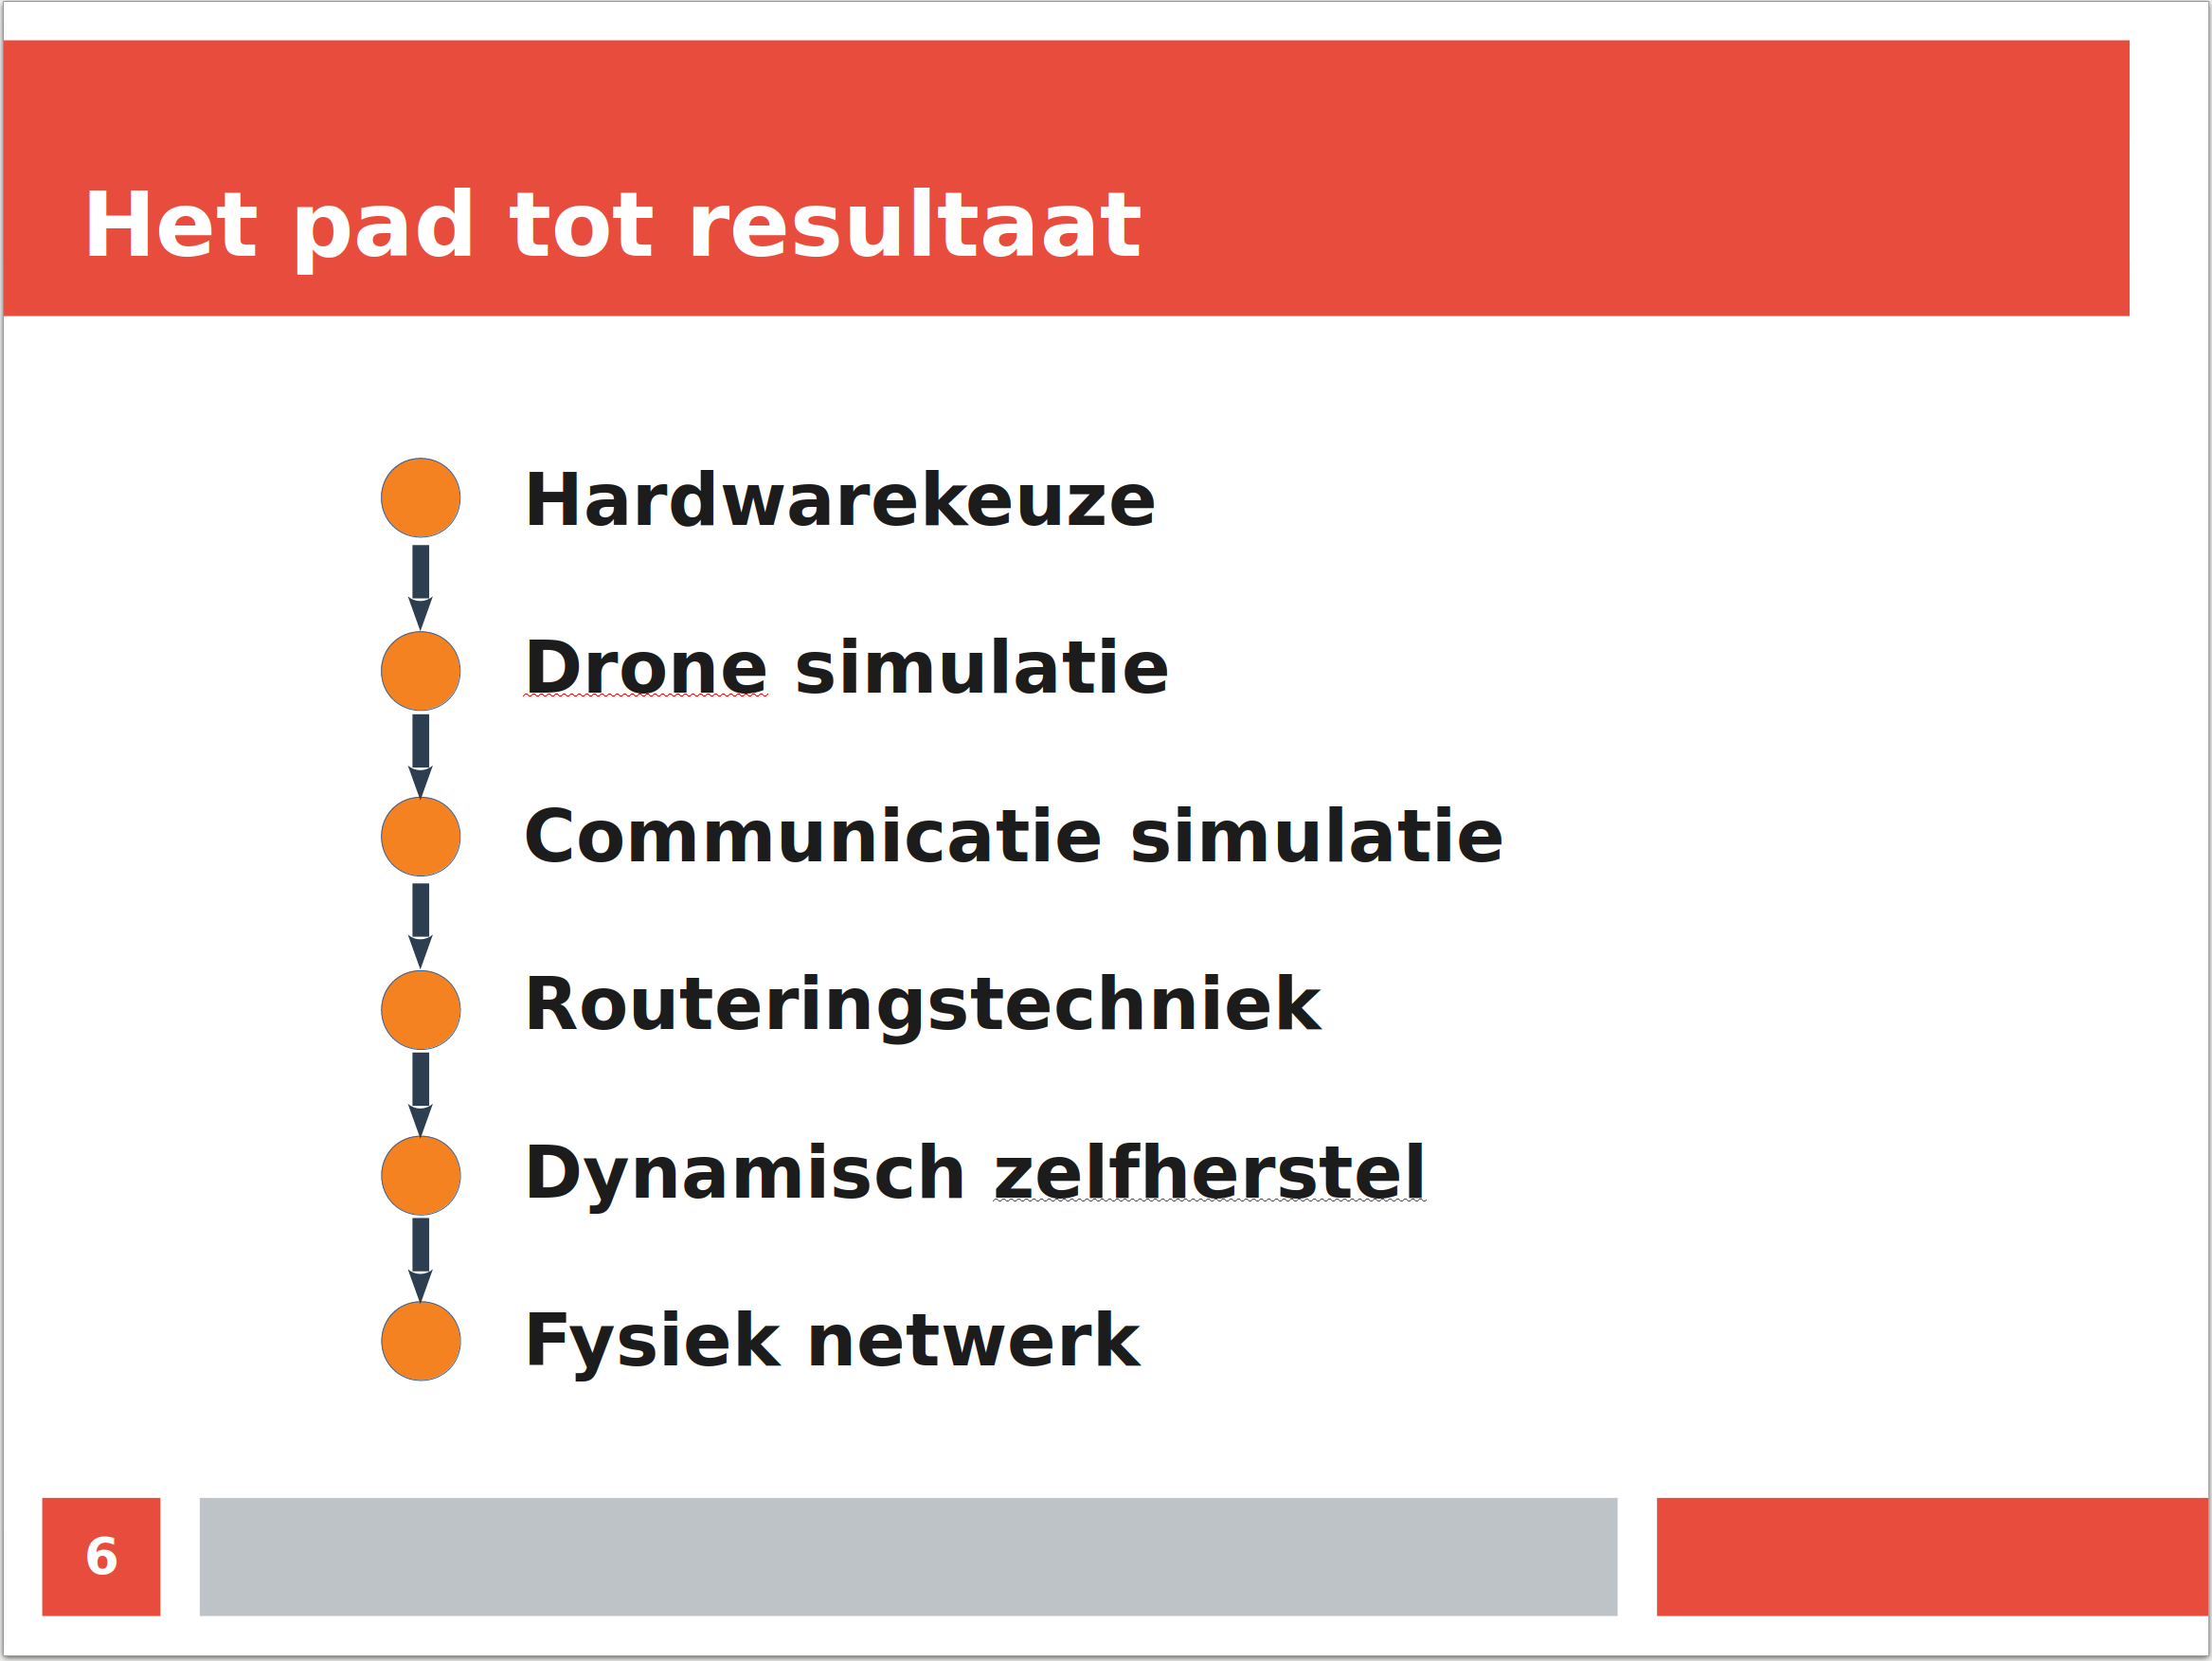
\includegraphics[width=5cm]{Afbeeldingen/Presentate1.png} }}%
	\qquad
	\subfloat[Slide waar de status van het pad bovenin zichtbaar is.]{{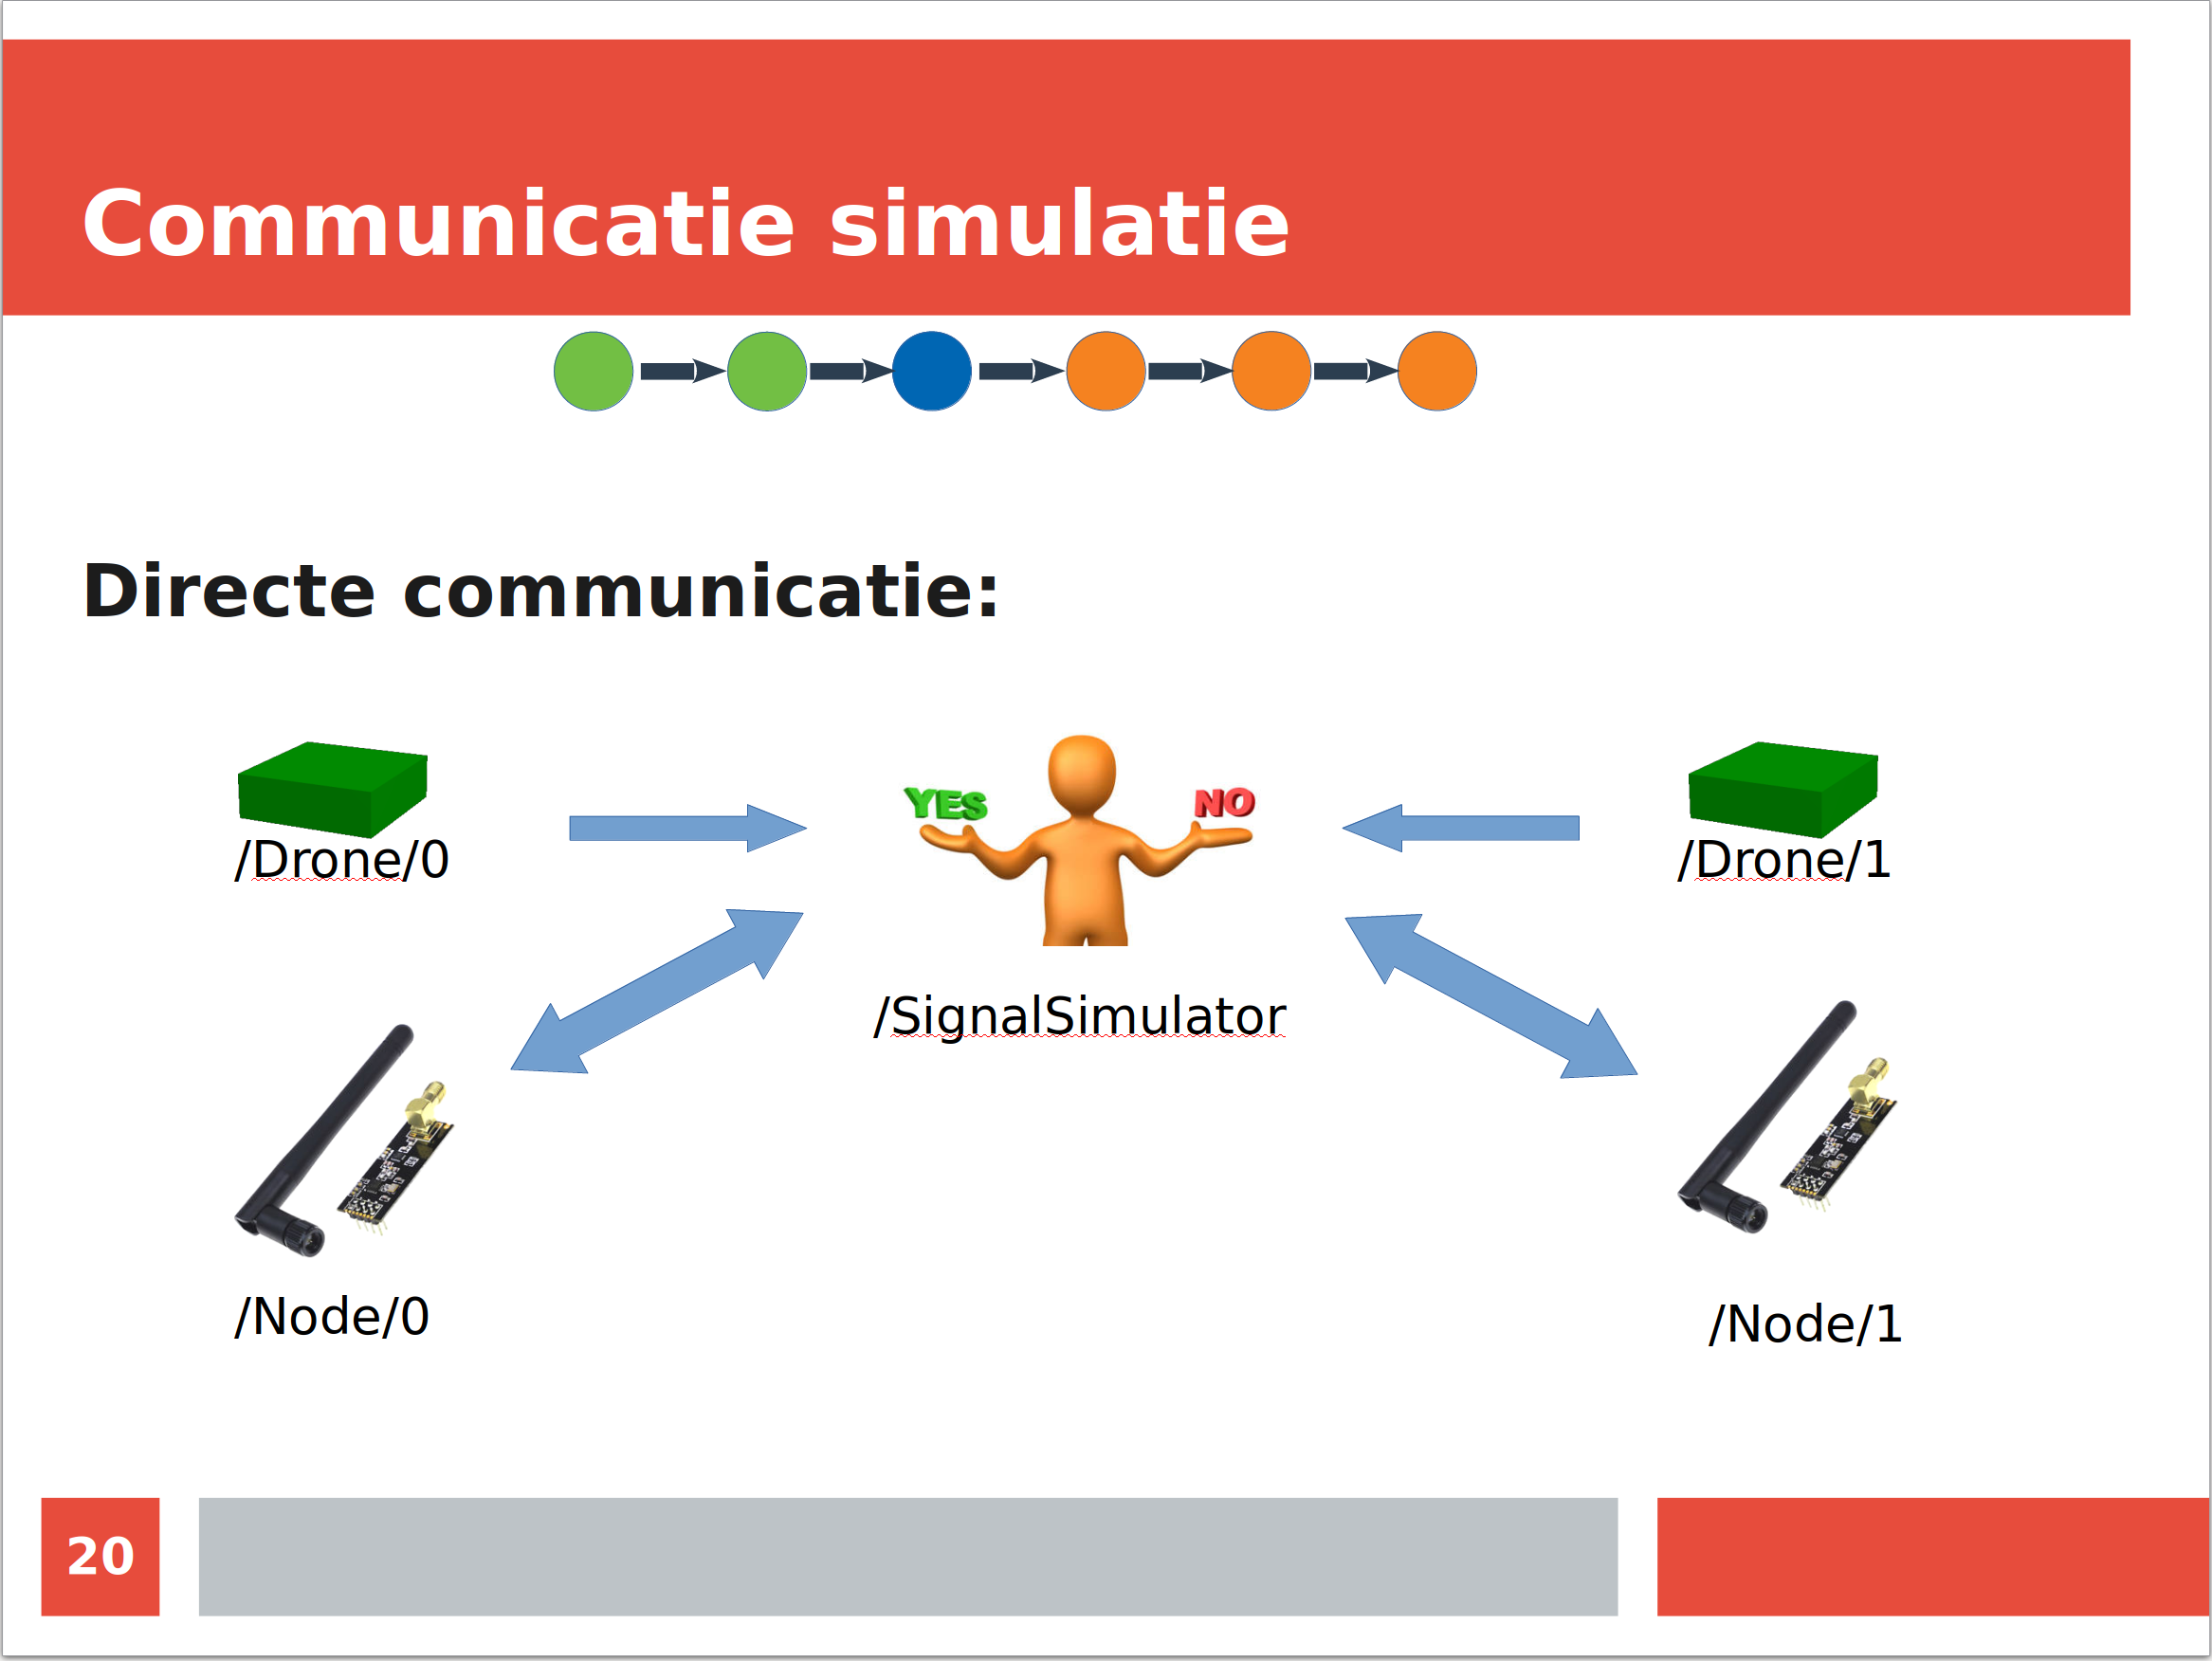
\includegraphics[width=5cm]{Afbeeldingen/Presentate2.png} }}%
	\caption{Slides uit de presentatie van de verdediging.}%
	\label{fig:vergelijkschermmen}%
\end{figure}

Het continue tonen van het pad bovenin de presentatie heb ik bedacht omdat ik het publiek wil meenemen op het pad die ik de afgelopen maanden heb bewandeld.
Een voordeel hieraan is dat het duidelijk is voor zowel mijzelf als het publiek waar we zijn in de presentatie.

\subsubsection{Contact met publiek (-[0], +[0], ++[7], leeg[2])}
Het contact met het publiek was volgens iedereen goed in orde.
Dit komt volgens hun omdat ik veel kennis had om goede inhoudelijke antwoorden te kunnen geven.  
Een tip die ik meekreeg was om bepaalde vragen voor te bereiden door ze in slides achter de presentaties te stoppen.

\subsection{Conclusie}

Op basis van de feedback kan ik concluderen dat ik het houden van de verdediging beheers.
Het is natuurlijk afwachten hoe het straks zal gaan tijdens de echte verdediging.
Veel kracht van de presentatie kwam uit de rust die ik kon bewaren.
De feedback geeft de laatste tips om de presentatie af te maken vooral de tip om slides voor mogelijke vragen toe te voegen vond ik handig.


\chapter{Conclusie}\label{sec:conclusie}
%Inhoudelijk, wat heeft het project opgeleverd, zet dat af tegen de doelstelling, heb je die gehaald?
%Afwijkingen beschrijven. Welke vervolgstappen kan het bedrijf nog nemen?
Het project heeft een geavanceerde simulator opgeleverd voor het testen van onderling communicerende drones.
Daarmee is het doel van het project behaald omdat Alten wil kunnen experimenteren in het opzetten van grootschalige netwerken door het gebruik van drones.
In de opgeleverde simulatie kunnen ze algoritmes testen voor verdelingen en beoordelen waar routers het meest belast zouden worden.

Naast de simulatie is er ook een prototype van het netwerkcomponent opgeleverd. 
De simulatie is gebouwd op basis van de eisen die de gekozen hardware opgelegd aan de software.
 
Door het gebruik van een interfaces kan er gemakkelijk geëxperimenteerd worden met de netwerkmodule.
In theorie kan er zelf getest worden met een fysieke antenne en een gesimuleerde drone zolang de gebruikte interfaces maar kloppen.

Het doel van Alten is om onderling verbonden drones te kunnen verdelen om zo een netwerk op te kunnen bouwen over een gebied.
Van te voren was al bekend dat de resultaten van dit project een eerste stap zijn naar het behalen van dit doel.
Het behaalde resultaat van het realistisch kunnen testen in een simulatie is de eerst die Alten nodig had voor deze eerste stap en die is bij deze dan ook behaald.

Het doel van de student om met dit project de vijf beroepscompetenties aan te tonen zijn ook behaald. Het vaststellen van de eisen aan het product in de \nameref{sec:software-requirements-specificatie} maar ook op andere plekken toont aan dat de student voldoet aan beoordelingscriteria 1. Het \nameref{sec:onderzoeksrapport} maar ook de keuzes vastgelegd in het \nameref{sec:software-design-document} laten zien dat de student voldoet aan beoordelingscriteria 2. Het \nameref{sec:software-design-document} samen met de opgeleverde \nameref{sec:broncode} laat zien dat de student bekwaam is in beoordelingscriteria 3. Het schrijven van een kwalitatief \nameref{sec:plan-van-aanpak} en het effectief kunnen bijsturen van het proces zoals omschreven in \nameref{sec:uitvoer-projectplan} laat zien dat de student bekwaam is in beoordelingscriteria 4.
Dit gehele verslag laat zien dat de studenten bekwaam is in het verantwoorden en reflecteren van zijn werk waarmee hij voldoet aan de laatste beoordelingscriteria 5.

\section{Advies vervolg project}\label{sec:advies-vervolg-project}
Wanneer dit project vervolgt wordt het volgende geadviseerd aan Alten:
\begin{itemize}
	\item Voorzie een volgende ontwikkelaar van een computer die een dedicated GPU aanwezig heeft zodat er grotere simulaties met gazebo gedraaid kunnen worden.
	
	\item Stel een buildserver voorzien van een geavanceerde code checker(Bijv. SonarQube of Coverity) beschikbaar.
	 
	\item Experimenteer met andere routeringsalgoritmes voordat er met fysieke netwerkapparatuur gewerkt gaat worden. Er bestaat niet één oplossing voor een dynamisch netwerk. Wellicht kan er geschakeld worden van protocol zodra de netwerkpunten statisch worden in de wereld.  
	
	\item Geef een volgende ontwikkelaar de ruimte om een geavanceerdere test omgeving op te zetten voor geautomatiseerde testen.
	Er kunnen scripts gemaakt worden om scenario's te testen in de verdeling van drones. Het gebruik van interface maakt het mogelijk de componenten los te testen door het gebruik van mocking.
	
	\item De draadloze communicatie is nu gebaseerd op onderlinge afstand tussen nodes. Het advies luidt om te onderzoeken of het haalbaar is met een simulatie met 100 communicatiepunten hier een andere techniek voor te gebruiken die bijvoorbeeld ook rekening kan houden met obstakels zodat er simulaties kunnen draaien in omgevingen met bijvoorbeeld bomen op gebouwen.
	
	\item Breidt de simulatie verder uit op basis van het gedrag van het fysieke netwerkcomponent die is opgeleverd. Focus hier op de communicatie van berichten, en hoe snel de netwerkmodule moet concluderen dat er geen verbinding mogelijk is.
	
	\item Schrijf de drone engine om naar het software patroon van een state machine en voeg een functie toe in de aangeboden interface die de staat van de drone aangeeft. Zo kan de netwerkmodule nog betere beslissingen nemen of bijvoorbeeld pas timers starten na het landen van de drone.
	
	\item Voordat de overstap gemaakt wordt van een abstracte drone naar een volledig gesimuleerde drone in de simulatie adviseer ik een uitbreiding tot een gesimuleerde drone die een batterijduur heeft.
	
\end{itemize}

\bibliographystyle{apacite}
\bibliography{bilbliography.bib}

\clearpage
\appendix
\chapter{Documenten}
Ter verantwoording van dit afstudeerverslag zijn de gemaakte documenten meegeleverd.
\section[Onderzoeksrapport Drone meshnetwerk simulatie]{Onderzoeksrapport Drone meshnetwerk simulatie.pdf}\label{sec:onderzoeksrapport-drone-meshnetwerk-simulatie}
Het onderzoekrapport.
\section[Plan van aanpak]{Plan van aanpak.pdf}\label{app:bijlage:plan-van-aanpak}
Het plan van aanpak.
\section[SoftwareDesignDocument]{SoftwareDesignDocument.pdf}\label{app:SoftwareDesignDocument}
Het software design document.
\section[SoftwareRequirementSpecification]{SoftwareRequirementSpecification.pdf}\label{app:softwarerequirementspecification}
Het software requirement specificatie.
\chapter{Broncode}\label{app:broncode}
Ter verantwoording van dit afstudeerverslag is de broncode opgeleverd en vinden in:

../Code/

\chapter{Resultaat CppCheck}\label{sec:resultaat-cppcheck}

\begin{center}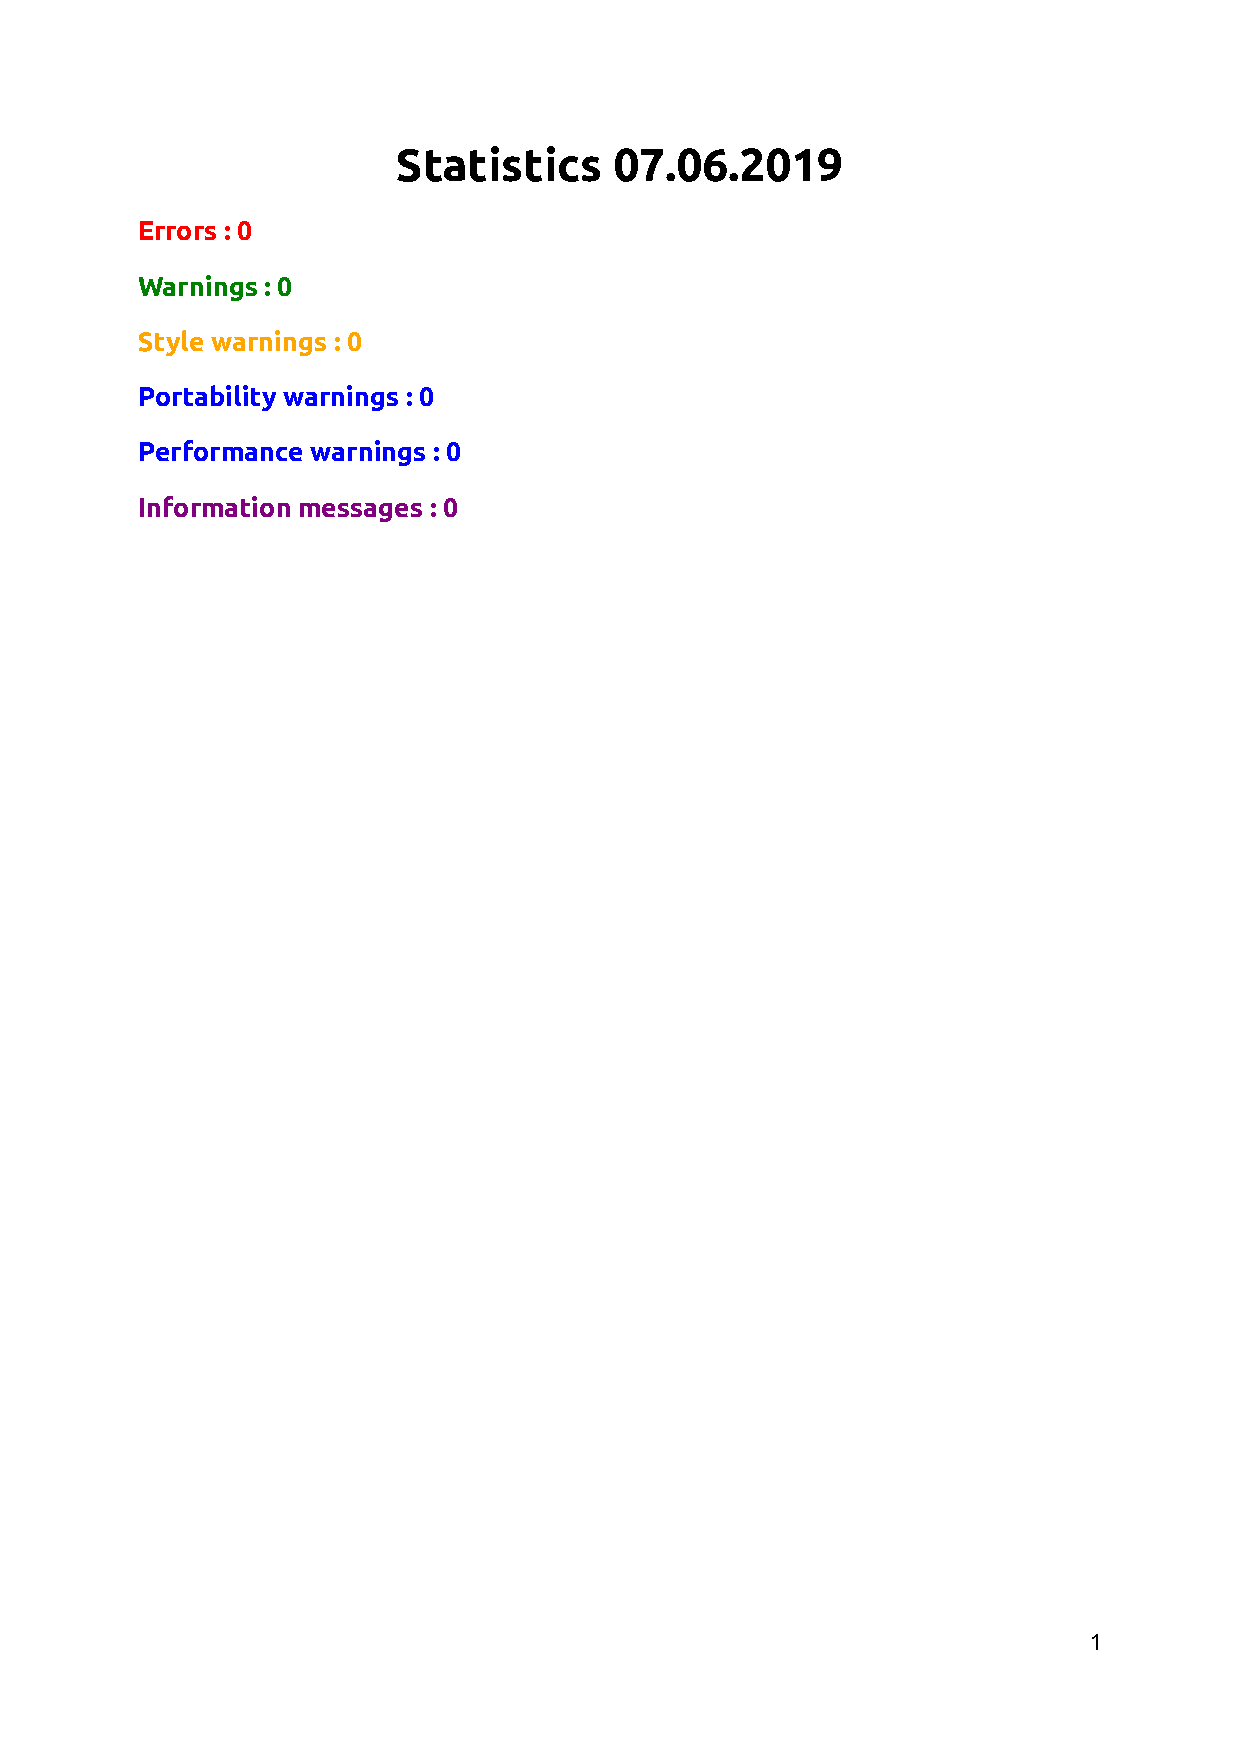
\includegraphics[page=1,width=.8\linewidth]{Bijlagen/cppcheck-gui.pdf}\end{center}
Te vinden in ./Bijlagen/.

\chapter{Resultaten GoogleTest}\label{sec:resultaten-googletest}
In deze bijlage zijn de resultaten van de Google Test toegevoegd.
Deze zijn te vinden in ./Bijlagen/test\textunderscore results/drone\textunderscore meshnetwork\textunderscore simulation/.



\section{gtest-drone\textunderscore meshnetwork\textunderscore simulation-GatewayDrone-test.xml}\label{sec:gtest-dronemeshnetworksimulation-gatewaydrone-testxml}
Bevat de testresultaten van het coderen en decoderen van de berichten die het netwerkcomponent gebruikt.

\section{gtest-drone\textunderscore meshnetwork\textunderscore simulation-HybridLMRoutingProtocol-test.xml}\label{sec:gtest-dronemeshnetworksimulation-hybridlmroutingprotocol-testxml}
Bevat de testresultaten van het routeringsprotocol.

\section{gtest-drone\textunderscore meshnetwork\textunderscore simulation-Vector3-test.xml}\label{sec:gtest-dronemeshnetworksimulation-vector3-testxml}
Bevat de testresultaten van de Vector3 template class.

\chapter{Templates}\label{app:templates}
Bevat template documenten te vinden in ./Templates/
\section{IterationAssessment.pdf}\label{app:IterationAssessment}
\section{Iteratieplan.pdf}\label{app:Iteratieplan}
\section{Usecase.pdf}\label{app:Usecase}


\chapter{Videos simulatie netwerkherstel door drone verplaatsing}\label{sec:videos-simulatie-netwerkherstel-door-drone-verplaatsing}
De video's van deze bijlagen zijn te vinden door het volgende pad te volgen: \newline
./Bijlagen/Videos simulatie netwerkherstel door drone verplaatsing/
\section{enkele verloren drone situatie 1.mp4}\label{sec:enkele-verloren-drone-situatie-1mp4} Video van een enkele drone die verbinding verliest en dit met een enkele stap weer opbouwt.
\section{enkele verloren drone situatie 2.mp4}\label{sec:enkele-verloren-drone-situatie-2mp4} Video van een enkele drone die verbinding verliest en nadat een enkele stap niet werkt weer terugkeert naar de gateway.
\section{groep verloren drones situatie 1.mp4}\label{sec:groep-verloren-drones-situatie-1mp4} Video van een groep verloren drones waarbij het terugzetten van een enkele stap van een drone verbinding weer herstelt.
\section{groep verloren drones situatie 2.mp4}\label{sec:groep-verloren-drones-situatie-2mp4} Video van een groep verloren drones waarbij twee drones een verplaatsing moeten uitvoeren voor het herstellen van het netwerk.
\section{groep verloren drones situatie 3.mp4}\label{sec:groep-verloren-drones-situatie-3mp4} Video waarbij alle werkende drones terug keren naar de gateway omdat er geen herstel wordt gevonden.

\chapter{Videos drone simulatie}\label{sec:videos-drone-simulatie}
Video's in ./Bijlagen/
%\section{gateway drone en 99 routerdrones.mp4}\label{sec:gateway-drone-en-99-routerdronesmp4}
%Video van 99 drones die verbinden met een gateway drone te vinden in:
\section{GatewayWissel.mp4}\label{sec:gatewaywisselmp4}
Video van drones die zich verspreiden, hier zijn twee gateways bij aanwezig.
Vervolgens wordt een essentieel punt uit gezet. 
De daarmee verbonden router wisselt van gateway. 

\chapter{Video fysiek hardware prototype}
Video's van het fysieke component.
Te vinden in ./Bijlagen/
\section{eerstecontact.mp4}\label{sec:eerstecontactmp4}
Video van fysieke routers die met elkaar communiceren.
\section{Fysieke router en drone.mp4}\label{sec:fysieke-router-en-dronemp4}
Video van fysieke router en gateway die verbinden met elkaar

\end{document}